\newpage
\chapter{Evaluation}
\label{chap:evaluation}

This section evaluates ALC as a compiler transformation by applying data permutation to a set of control-divergent loops and comparing its effectiveness to previous implementations of ALC and to code generated by existing production compilers. 
This evaluation aims to answer the following questions:

\noindent\circled{1} Can Data Permutation improve ALC performance by reducing memory stalls?

\noindent\circled{2} Do scatter instructions impact ALC's performance?

\noindent\circled{3} Should ALC be applied on loops with a single \cpath?

The results indicate that data permutation leads to a significant speedup of up to 79\% over \ifconverted code and outperforms state-of-the-art compiler-based approaches.

\section{Setup}
\label{sec:setup}

The experiments run on a machine equipped with a Fujitsu A64FX locked at $1.8$GHz that has access to 32GiB of RAM and runs Rocky Linux (release 8.4).
A64FX is the first processor that implements ARMv8.2-A SVE instruction and it operates with 512-bit vector registers.
The evaluation micro-benchmarks were developed in-house and are written in the C language.
Each micro-benchmark is designed to be representative of application code and to ease the identification and measurement of factors that impact the performance of both \ifconverted code and ALC-transformed code.
Wyatt \etal seminal work predicted the performance of ALC using hand-modified versions of applications in the SPEC CPU2017 benchmark suite running on a functional simulator~\cite{spec}.
Those modifications included removing control-flow dependent paths that execute I/O operations --- a transformation that cannot be safely implemented in a compiler because it alters the behavior of the program.
This thesis aims to evaluate the automated generation of ALC code by a compiler transformation pass and thus can only be applied to programs to which the compiler can safely apply ALC without user intervention.
The micro-benchmarks used in this evaluation are comprehensive and share characteristics with loops found in the SPEC CPU2017 benchmark Suite.
The limitations and challenges of the current ALC implementation are discussed in \rsec{eval-limitations}.

The evaluation micro-benchmarks consist of loops that contain either an \code{if-then-else} or  a single \code{if} statement.
Two micro-benchmarks help understand the impact of the factors discussed in \rsec{alc-analysis}:
\begin{inparaenum}
    \item \textbf{\ifElseBench} contains a loop that executes $N$ times with two \cpaths in its body. Each \cpath has: $20$ arithmetic, $2$ load, and $3$ store instructions;
    \item \textbf{\ifThenBench} also contains a loop that executes $N$ times but with a single \cpath, which has: $20$ arithmetic, $2$ load, and $3$ store instructions.
\end{inparaenum}
$N$ is set to five million for all experiments.
Complete source code of ALC's LLVM IR pass and evaluation micro-benchmarks is available as part of this thesis \textbf{ARTIFACT}\footnote{\href{https://github.com/Rouzbeh99/Active-Lane-Consolidation.git}{e8700cb320f3942eb3dfc9a585587167243a086d}}.
All source code is compiled with Clang/LLVM version 15.0.0\footnote{\href{https://github.com/llvm/llvm-project/commit/61baf2ffa7071944c00a0642fdb9ff77d9cff0da}{61baf2ffa7071944c00a0642fdb9ff77d9cff0da}} and highest optimization level enabled (\code{-O3}).

\section{Experimental Methodology}
\label{sec:methodology}

Results presented in the following sections are the average of one hundred executions of each program.
Very little variation was observed between measurements.
Performance metrics were collected using \acrshort{papi} library version $7.0.0$\footnote{\href{https://bitbucket.org/icl/papi/commits/c415d2f1190027c961c904a4305b3eeaacce3df2}{c415d2f1190027c961c904a4305b3eeaacce3df2}}~\cite{papi}.
The performance for each micro-benchmark is measured with varied \textbf{input sparsity}, the percentage of loop iterations in which the control-flow condition evaluates to true.
Results are reported for input sparsity of $2\%$, $20\%$, $40\%$, and $80\%$, with true predicates randomly distributed throughout the loop iterations.
These percentages represent use cases varying from very few active lanes ($2\%$) to mostly active lanes ($80\%$).
A random distribution of true predicates means that none of the evaluated approaches can make assumptions about the order or the pattern of taken/not-taken paths.
To Apply ALC, input source code is first compiled to LLVM IR using Clang. The  produced IR is fed to the transformation pass and all analyses and transformations are done at this level. Then clean up and further optimization passes in the \code{O3} pipeline are executed to ensure that the transformed IR is fully optimized. 
Finally, the generated binary file is produced. The process is shown in \rfig{compile-process}.


\begin{figure*}[t]
  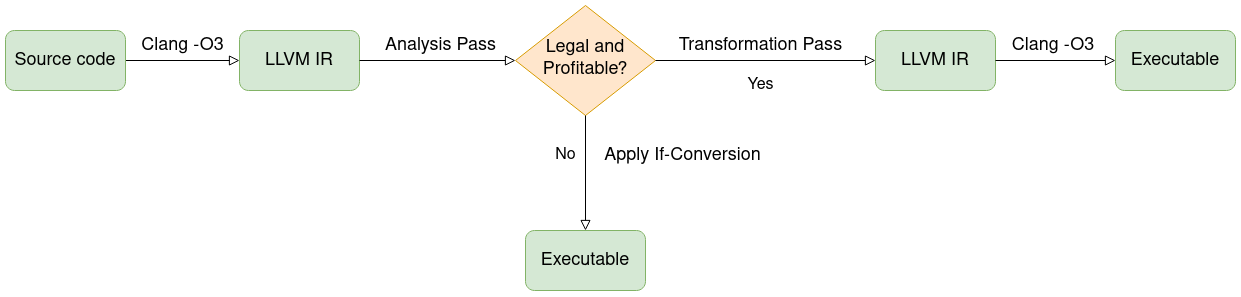
\includegraphics[width=1.05\textwidth, height=.21\textheight]{Figures/Evaluations/Compilation Process.png}
  \caption{Compilation process}
  \label{fig:compile-process}
\end{figure*}



The results presented next contrast the performance of:
\begin{inparaenum}[(i)]
  \item \textbf{\ALC}, a compiler-generated version of Wyatt \etal's ALC;
  \item \textbf{\ALCdp}, the improved version of \ALC proposed in this thesis which employs data permutation to eliminate gather instructions;
  \item \textbf{\ifconv}, \ifconversion performed by Arm's Clang compiler.
\end{inparaenum}
A comparison of the \ifconversion code generated by three production-ready compilers --- Arm's Clang, \acrshort{gcc}, and Clang --- revealed that Arm's Clang generates slightly faster code for the evaluated micro-benchmarks.


\section{Data Permutation: More Instructions But Better Performance}
\label{sec:data-permutation-evaluation}



This experiment aims to answer \circled{1} by comparing the performance of each version of the \ifElseBench micro-benchmark generated by Clang.

\begin{figure*}[t]
  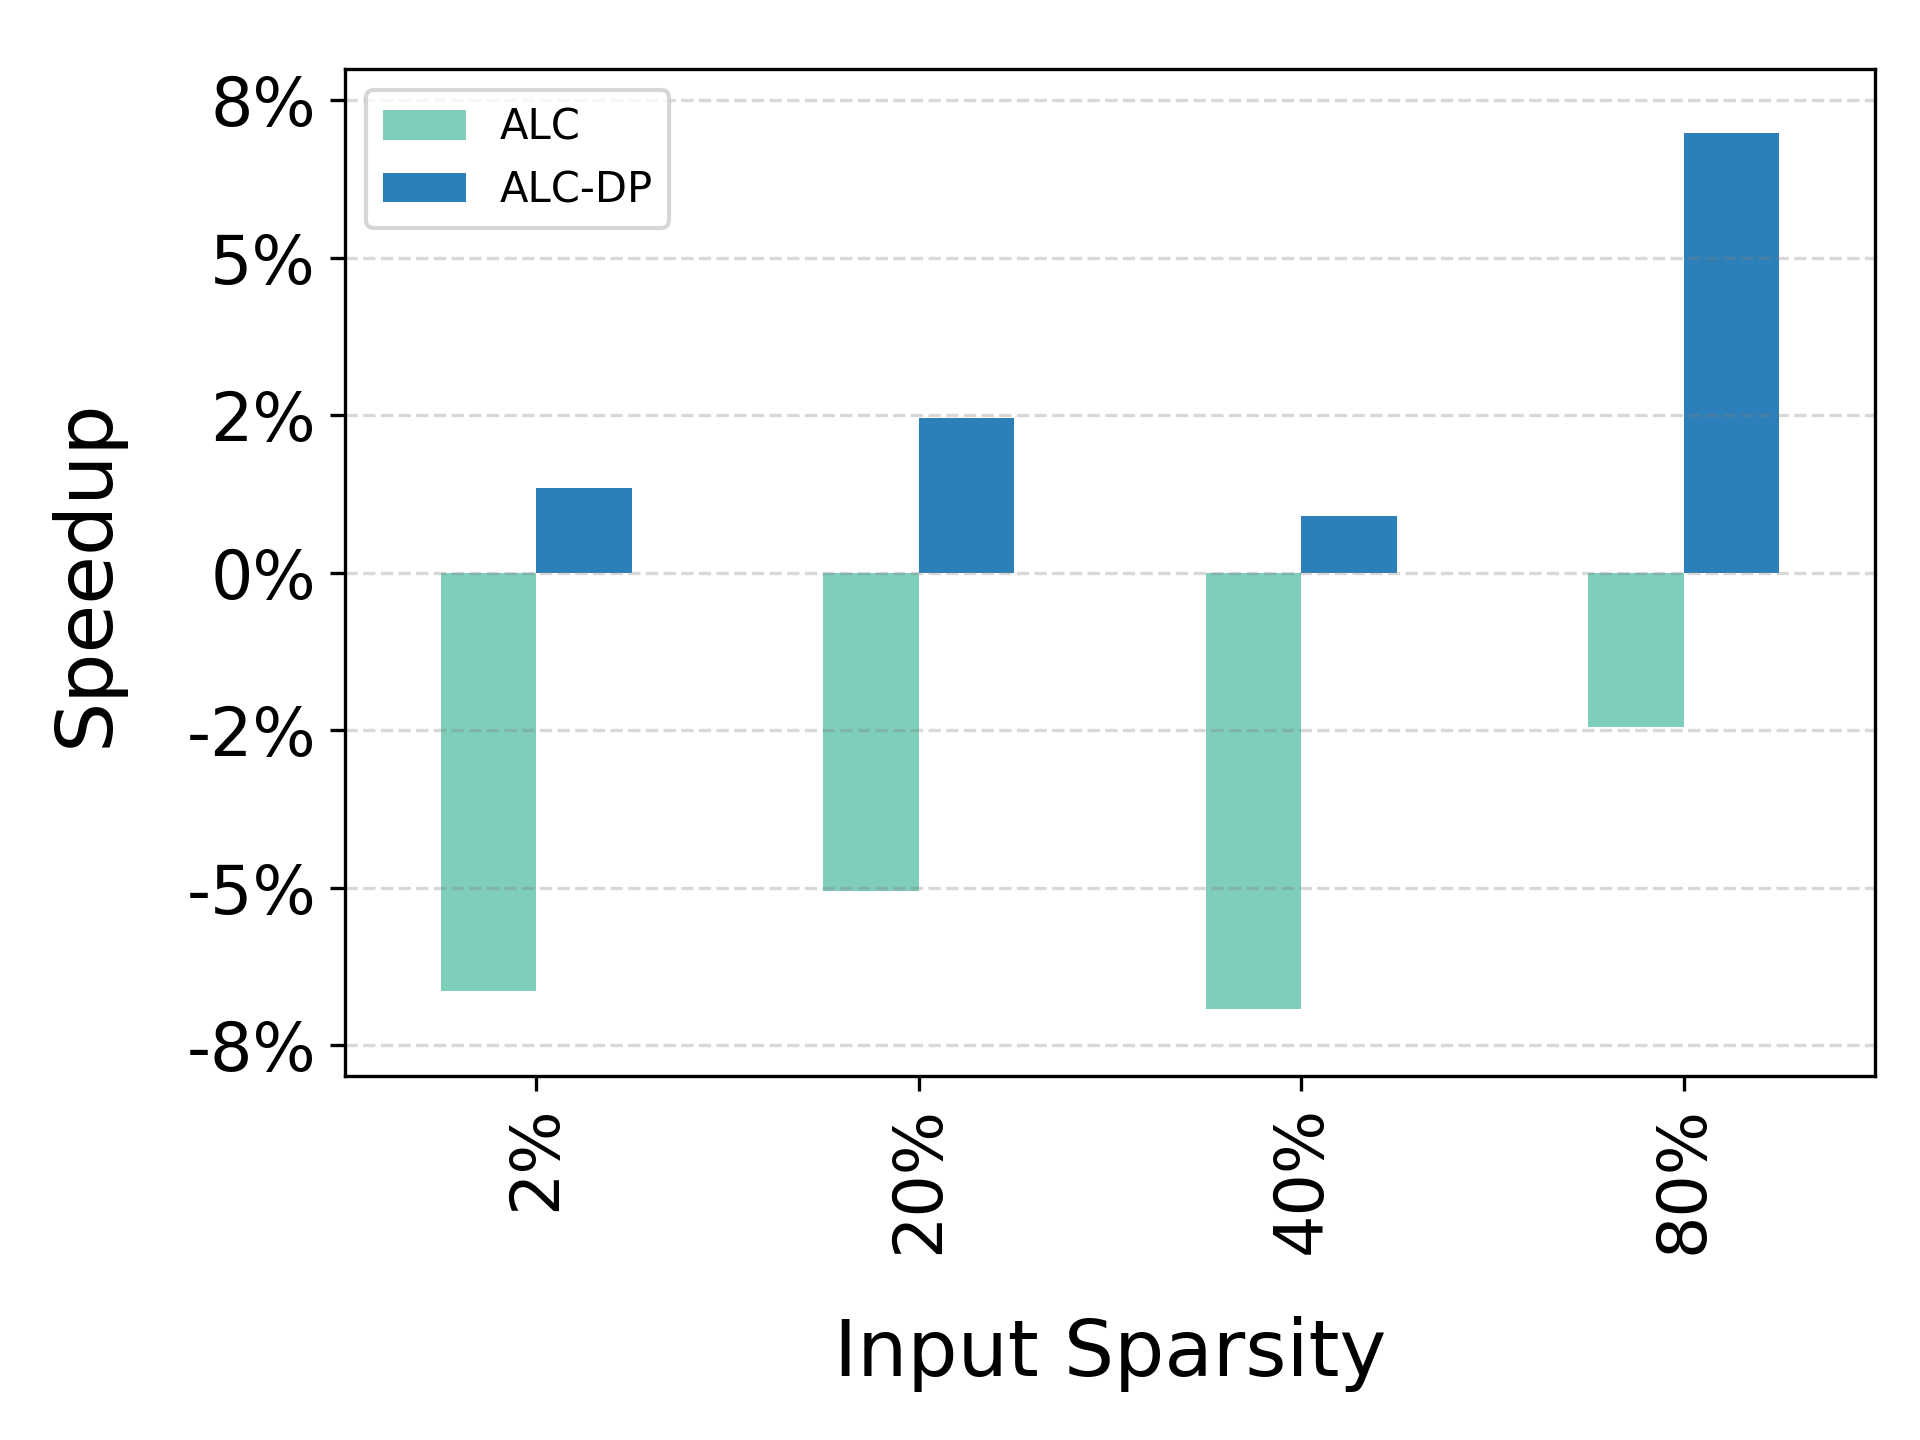
\includegraphics[width=0.8\textwidth]{Figures/Evaluations/if_then_else_many_scatter_speedup.png}
  \caption{ALC and Data Permutation speedups over If-Conversion for \ifElseBench micro-benchmark that has two CFDPs.}
  \label{fig:if-then-else-many-scatter-speedup}
\end{figure*}

\begin{figure*}[h!]
  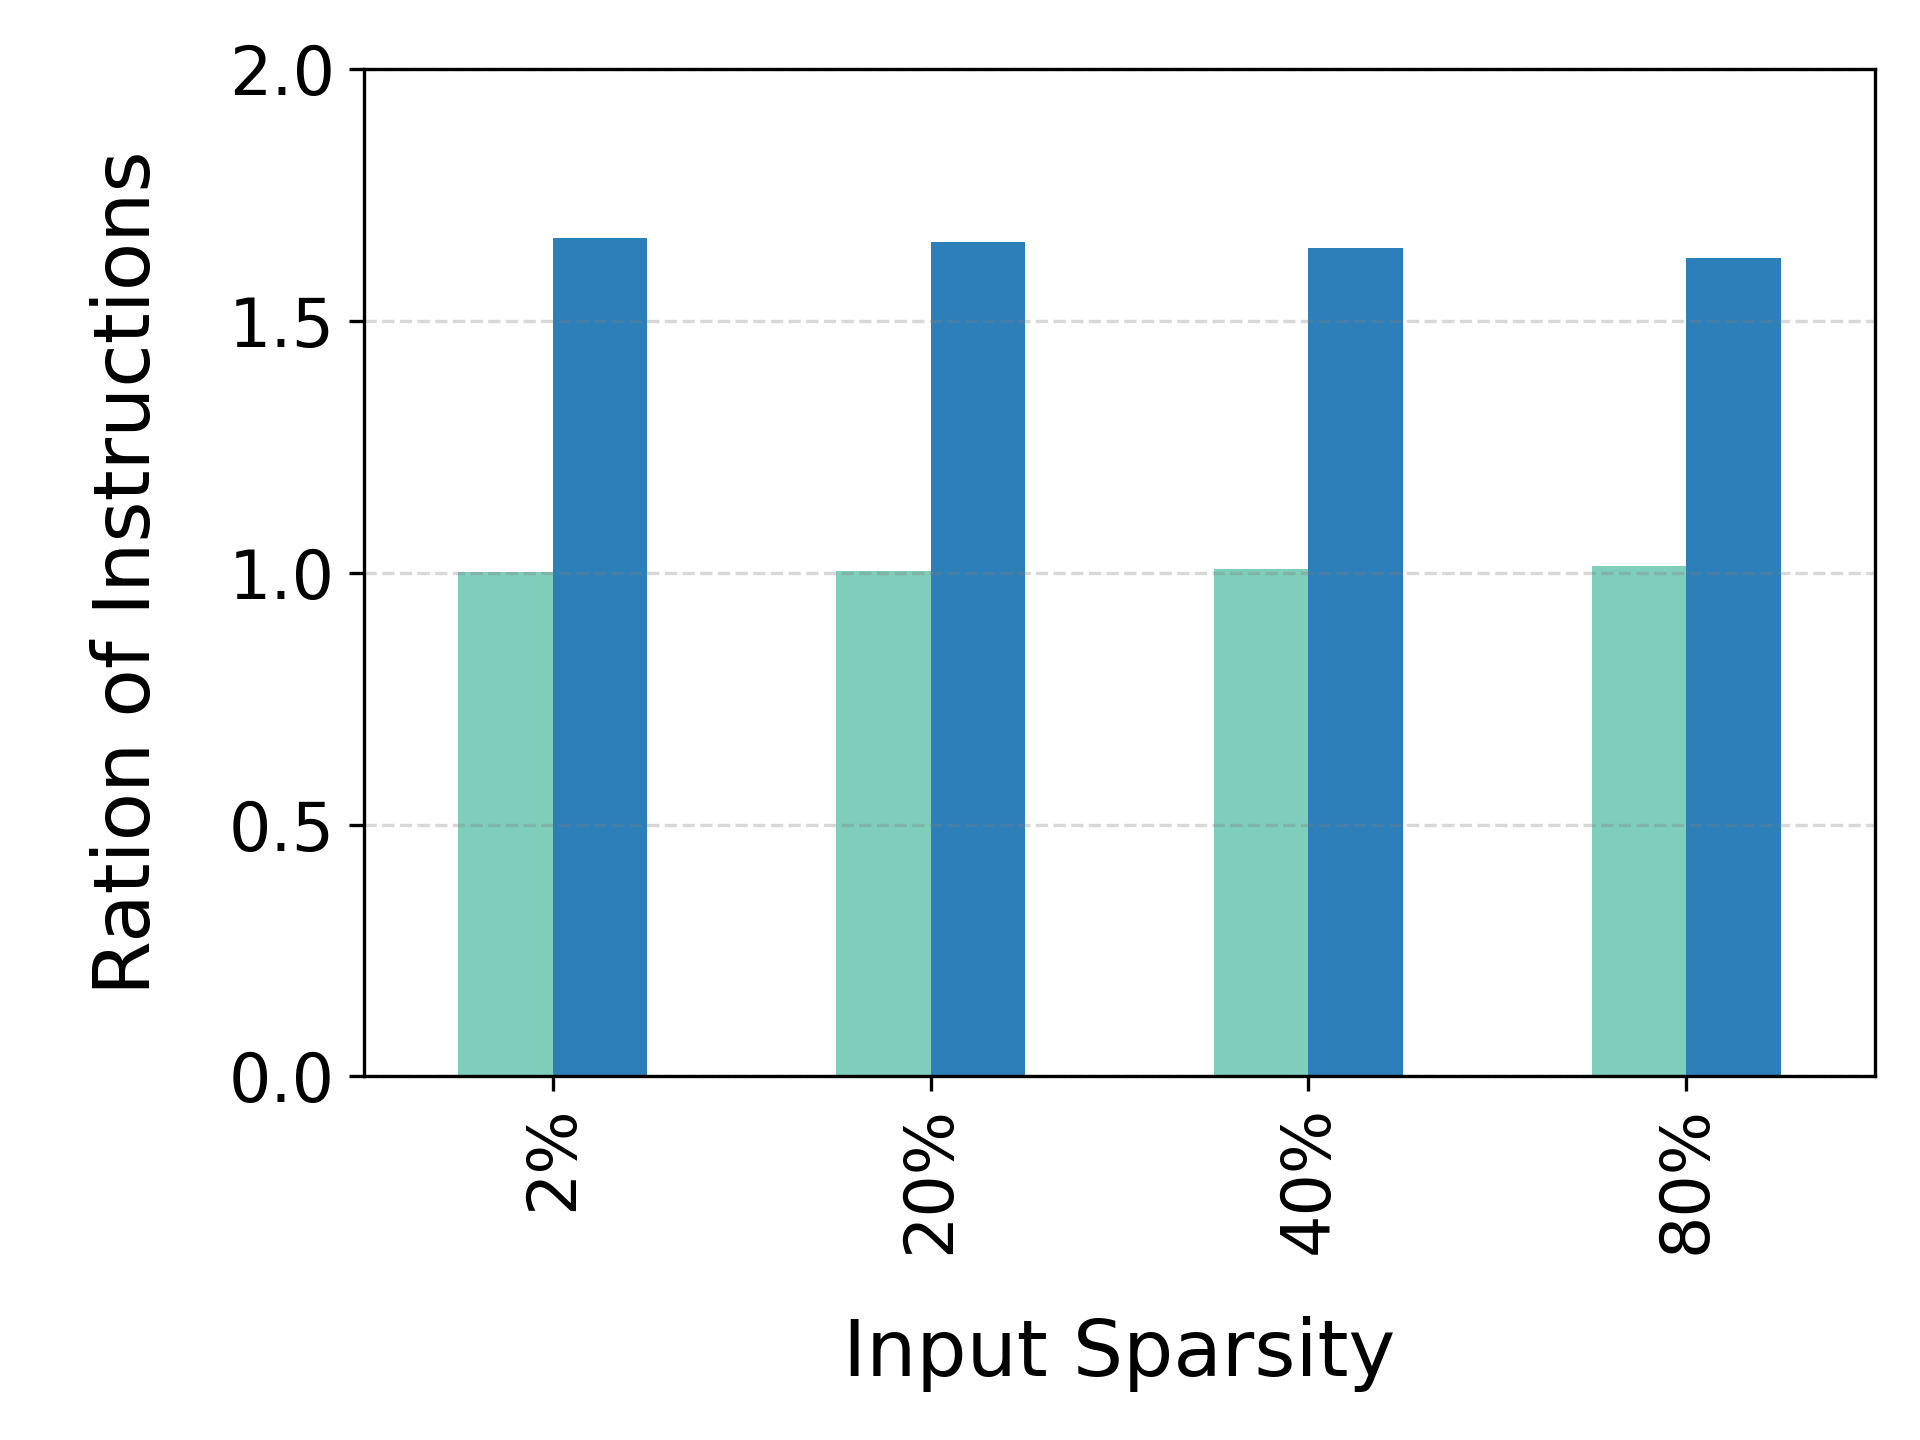
\includegraphics[width=0.8\textwidth]{Figures/Evaluations/if_then_else_many_scatter_instr.png}
  \caption{Ratio of dynamically executed instructions}
  \label{fig:if-then-else-many-scatter-inst}
\end{figure*}

\begin{figure*}[htbp]
  \centering
  \begin{subfigure}{4 cm}
    \centering
    
\includegraphics[width=\textwidth]{Figures/Evaluations/Legend.png}
  \end{subfigure}\\
  
  \begin{subfigure}{.49\textwidth}
    \centering
    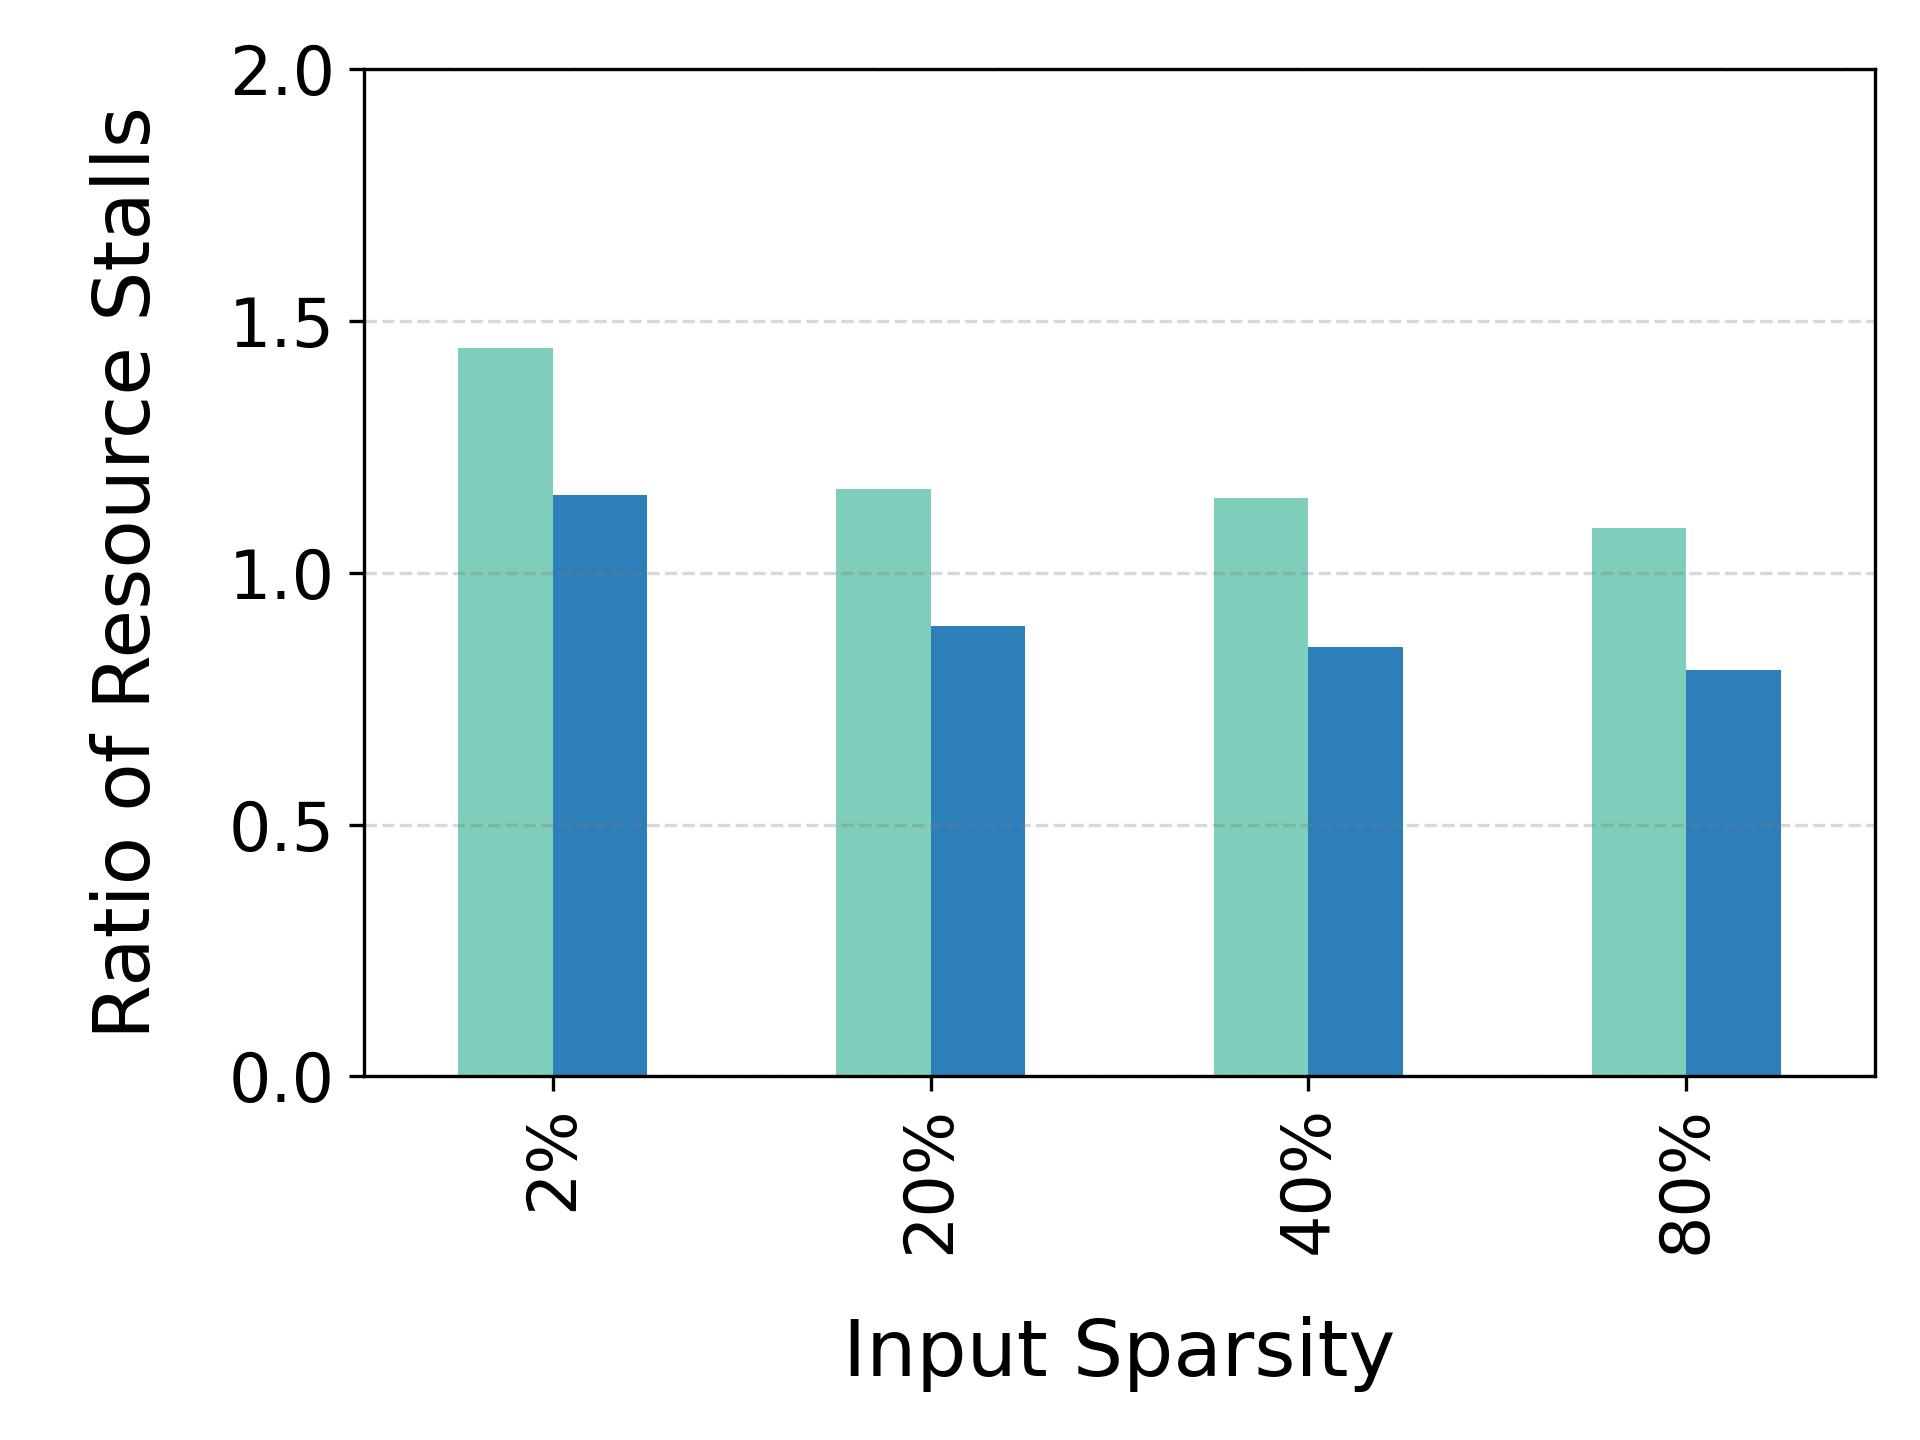
\includegraphics[width=\textwidth, height=.28\textheight]{Figures/Evaluations/if_then_else_many_scatter_resource_stalls.png}
    \caption{Ratio of resource-busy stalls.}
    \label{fig:if-then-else-many-scatter-resource-stalls}
  \end{subfigure}%
  \begin{subfigure}{.49\textwidth}
        \centering
    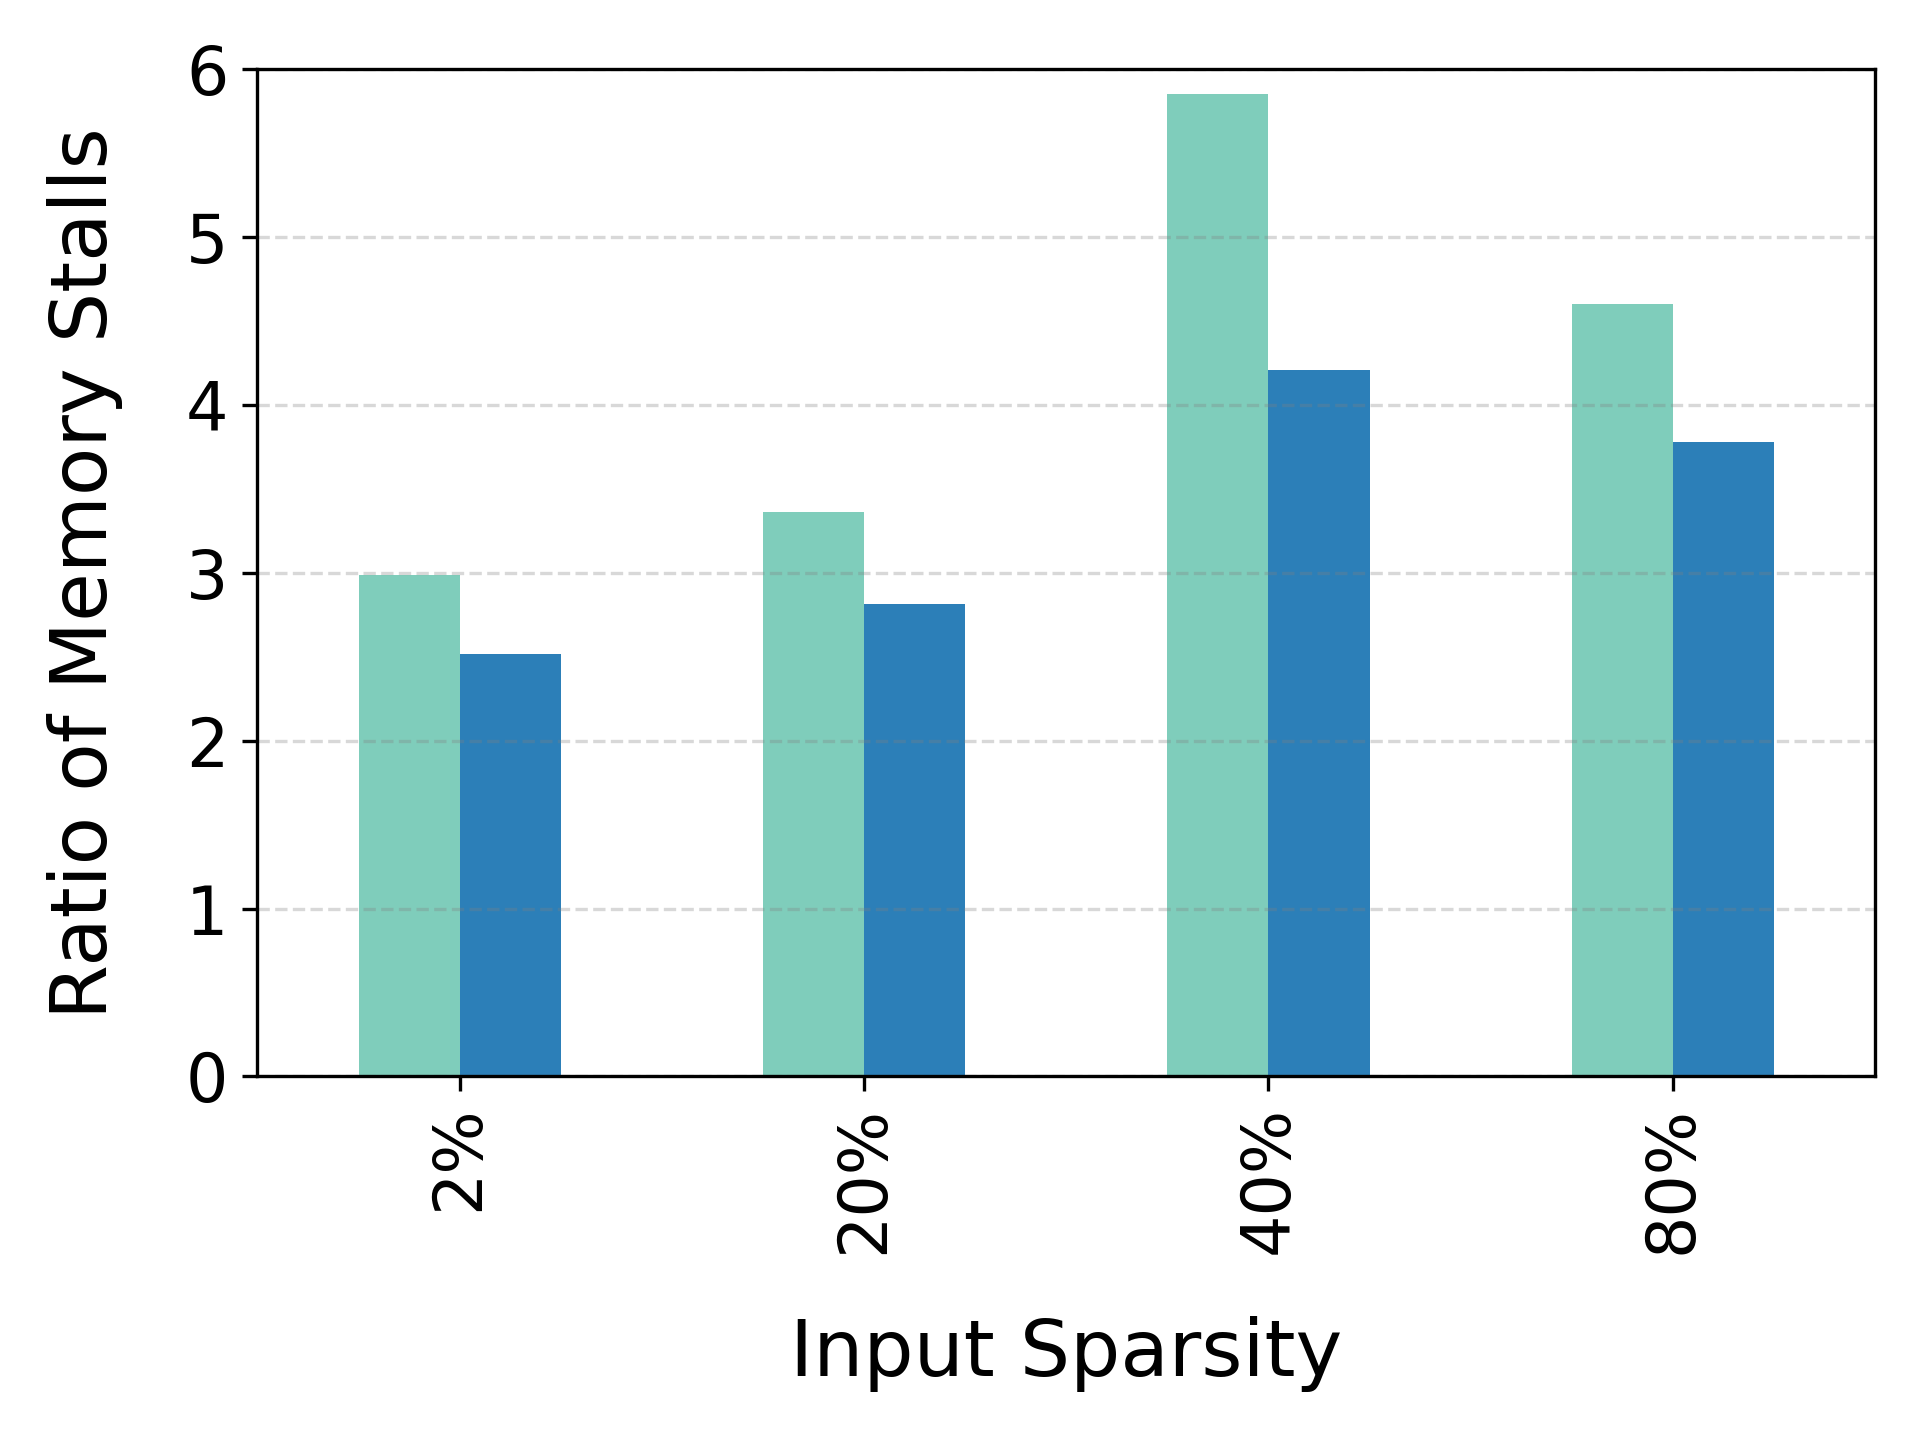
\includegraphics[width=\textwidth, height=.28\textheight]{Figures/Evaluations/if_then_else_many_scatter_mem_stalls.png}
    \caption{Ratio of memory-induced stalls.}
    \label{fig:if-then-else-many-scatter-mem-stalls}
  \end{subfigure}%
  \caption{Evaluation of the \ifElseBench micro-benchmark that has two CFDPs. All metrics are normalized with respect to \ifconverted code (\ifconv).}
\end{figure*}


\rfig{if-then-else-many-scatter-speedup} shows the speedup over \ifconv.
As discussed in \rsec{gathers-scatters-are-bad}, gather instructions have higher latency than regular vector loads, thus hurting \ALC's performance in comparison to \ifconv, which only uses regular vector load instructions.
Such overhead is quantified in \rfig{if-then-else-many-scatter-mem-stalls}, which indicates that the ratio of stalls due to pending memory operations (w.r.t \ifconv) is significantly higher in \ALC than in \ALCdp, which explains \ALCdp better performance.
Also, the address calculations of gather/scatter instructions are executed in the vector units and thus compete for resources and stall other arithmetic operations in \ifElseBench.
As \rfig{if-then-else-many-scatter-resource-stalls} indicates, \ALC has more stalls waiting for resources than the baseline \ifconv while \ALCdp has fewer resource stalls than \ALC because gather instructions are eliminated via data permutation.
In addition, \ALCdp outperforms \ifconv for all input sparsity cases and, in particular, by more than $7\%$ in the $80\%$ sparsity case --- a positive answer to question \circled{1}.
\ALCdp performs better than \ifconv even though it executes more instructions to perform data permutation,  as \rfig{if-then-else-many-scatter-inst} indicates.
These data-permutation instructions are vector-to-vector instructions that incur much lower latency than gather instructions do.
\ALCdp still suffers more memory stalls than the baseline \ifconv because of the high latency of scatter stores that, usually, cannot be avoided.
In contrast,  \ALC always performs worse than \ifconv and shows performance degradation of up to $6\%$ in the $40\%$ sparsity case.

\section{Scatter Instructions Significantly Impact Performance}
\label{sec:eval-scatters-costs}


\begin{figure*}[t]
  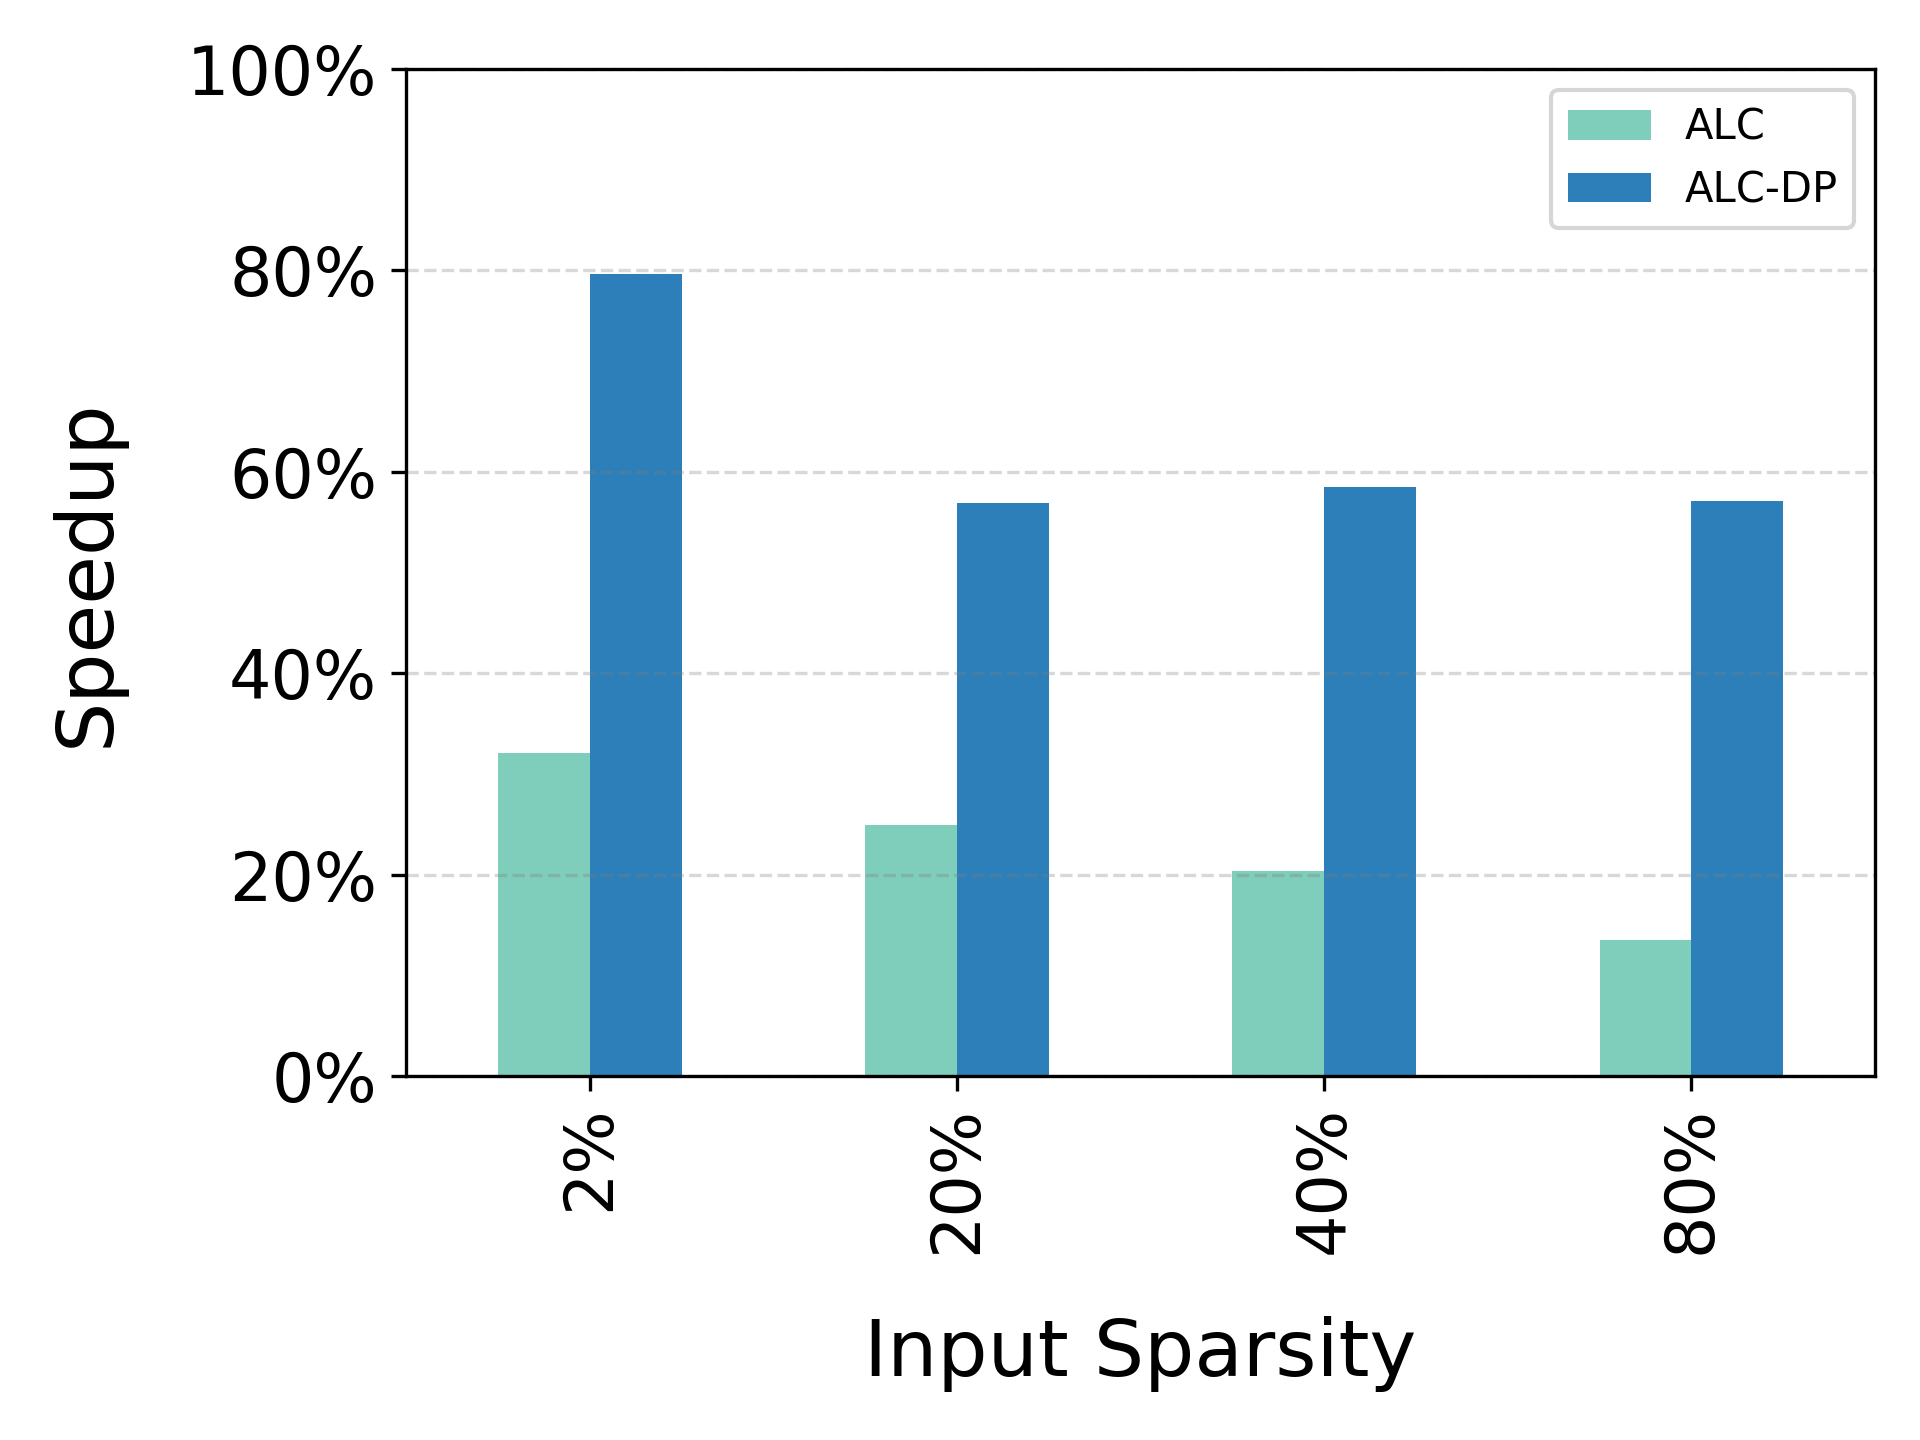
\includegraphics[width=0.8\textwidth]{Figures/Evaluations/if_then_else_few_scatter_speedup.png}
  \caption{Data Permutation and ALC Speedups in the presence of fewer Scatter instructions}
  \label{fig:if-then-else-few-scatter-speedup}
\end{figure*}

\begin{figure*}[t]
  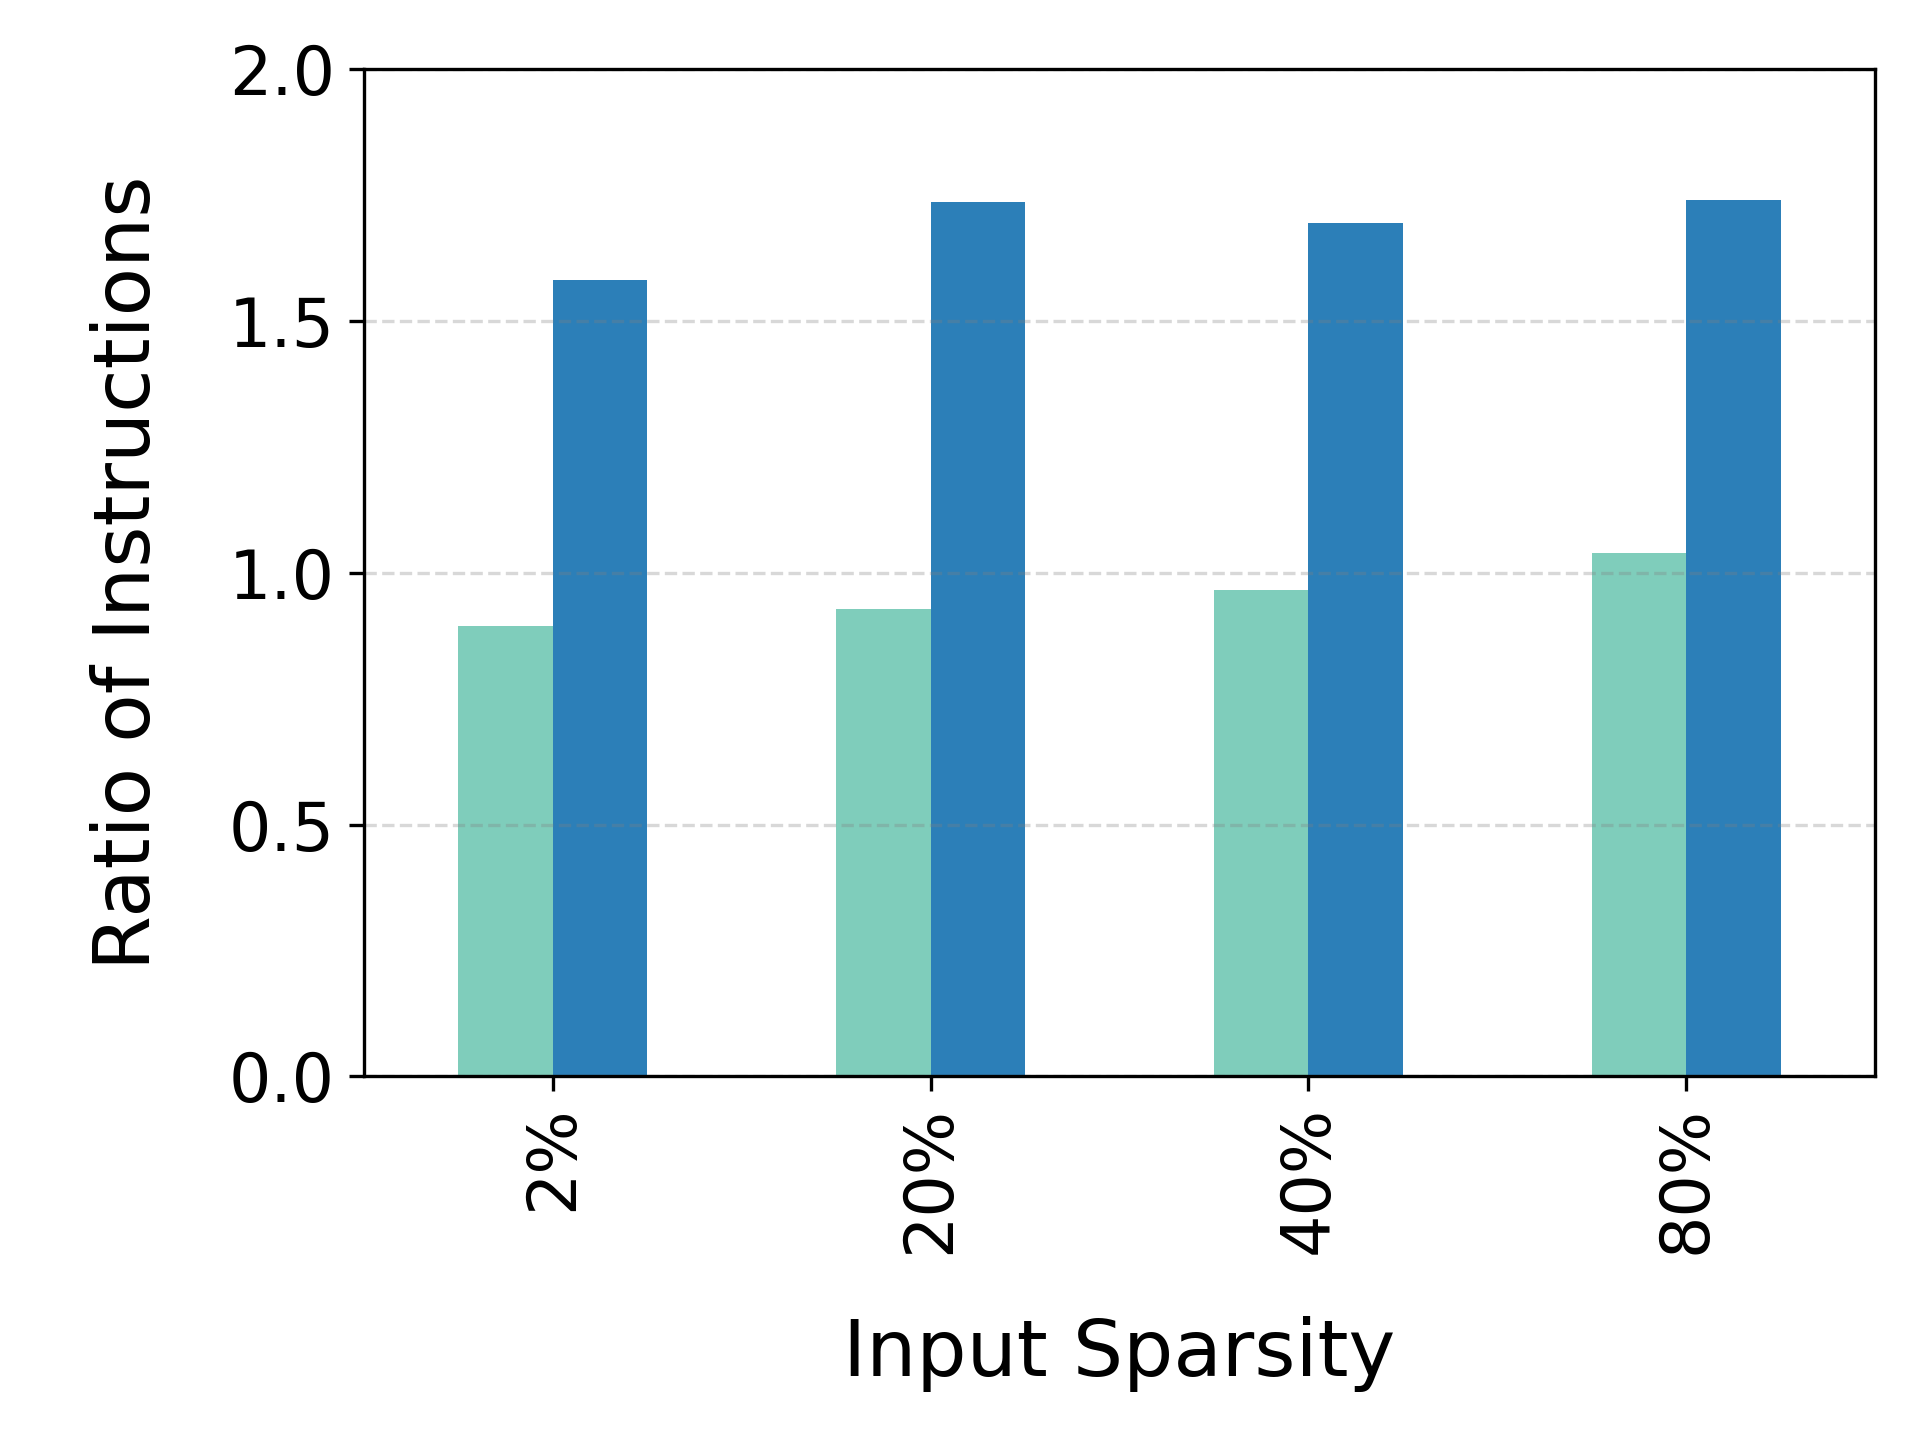
\includegraphics[width=0.8\textwidth]{Figures/Evaluations/if_then_else_few_scatter_instr.png}
  \caption{Ratio of dynamically executed instructions}
  \label{fig:if-then-else-few-scatter-inst}
\end{figure*}

\begin{figure*}[htbp]
  \centering
 \begin{subfigure}{4cm}
    \centering
    
\includegraphics[width=\textwidth]{Figures/Evaluations/Legend.png}
 \end{subfigure}\\
  \begin{subfigure}{.5\textwidth}
    \centering
    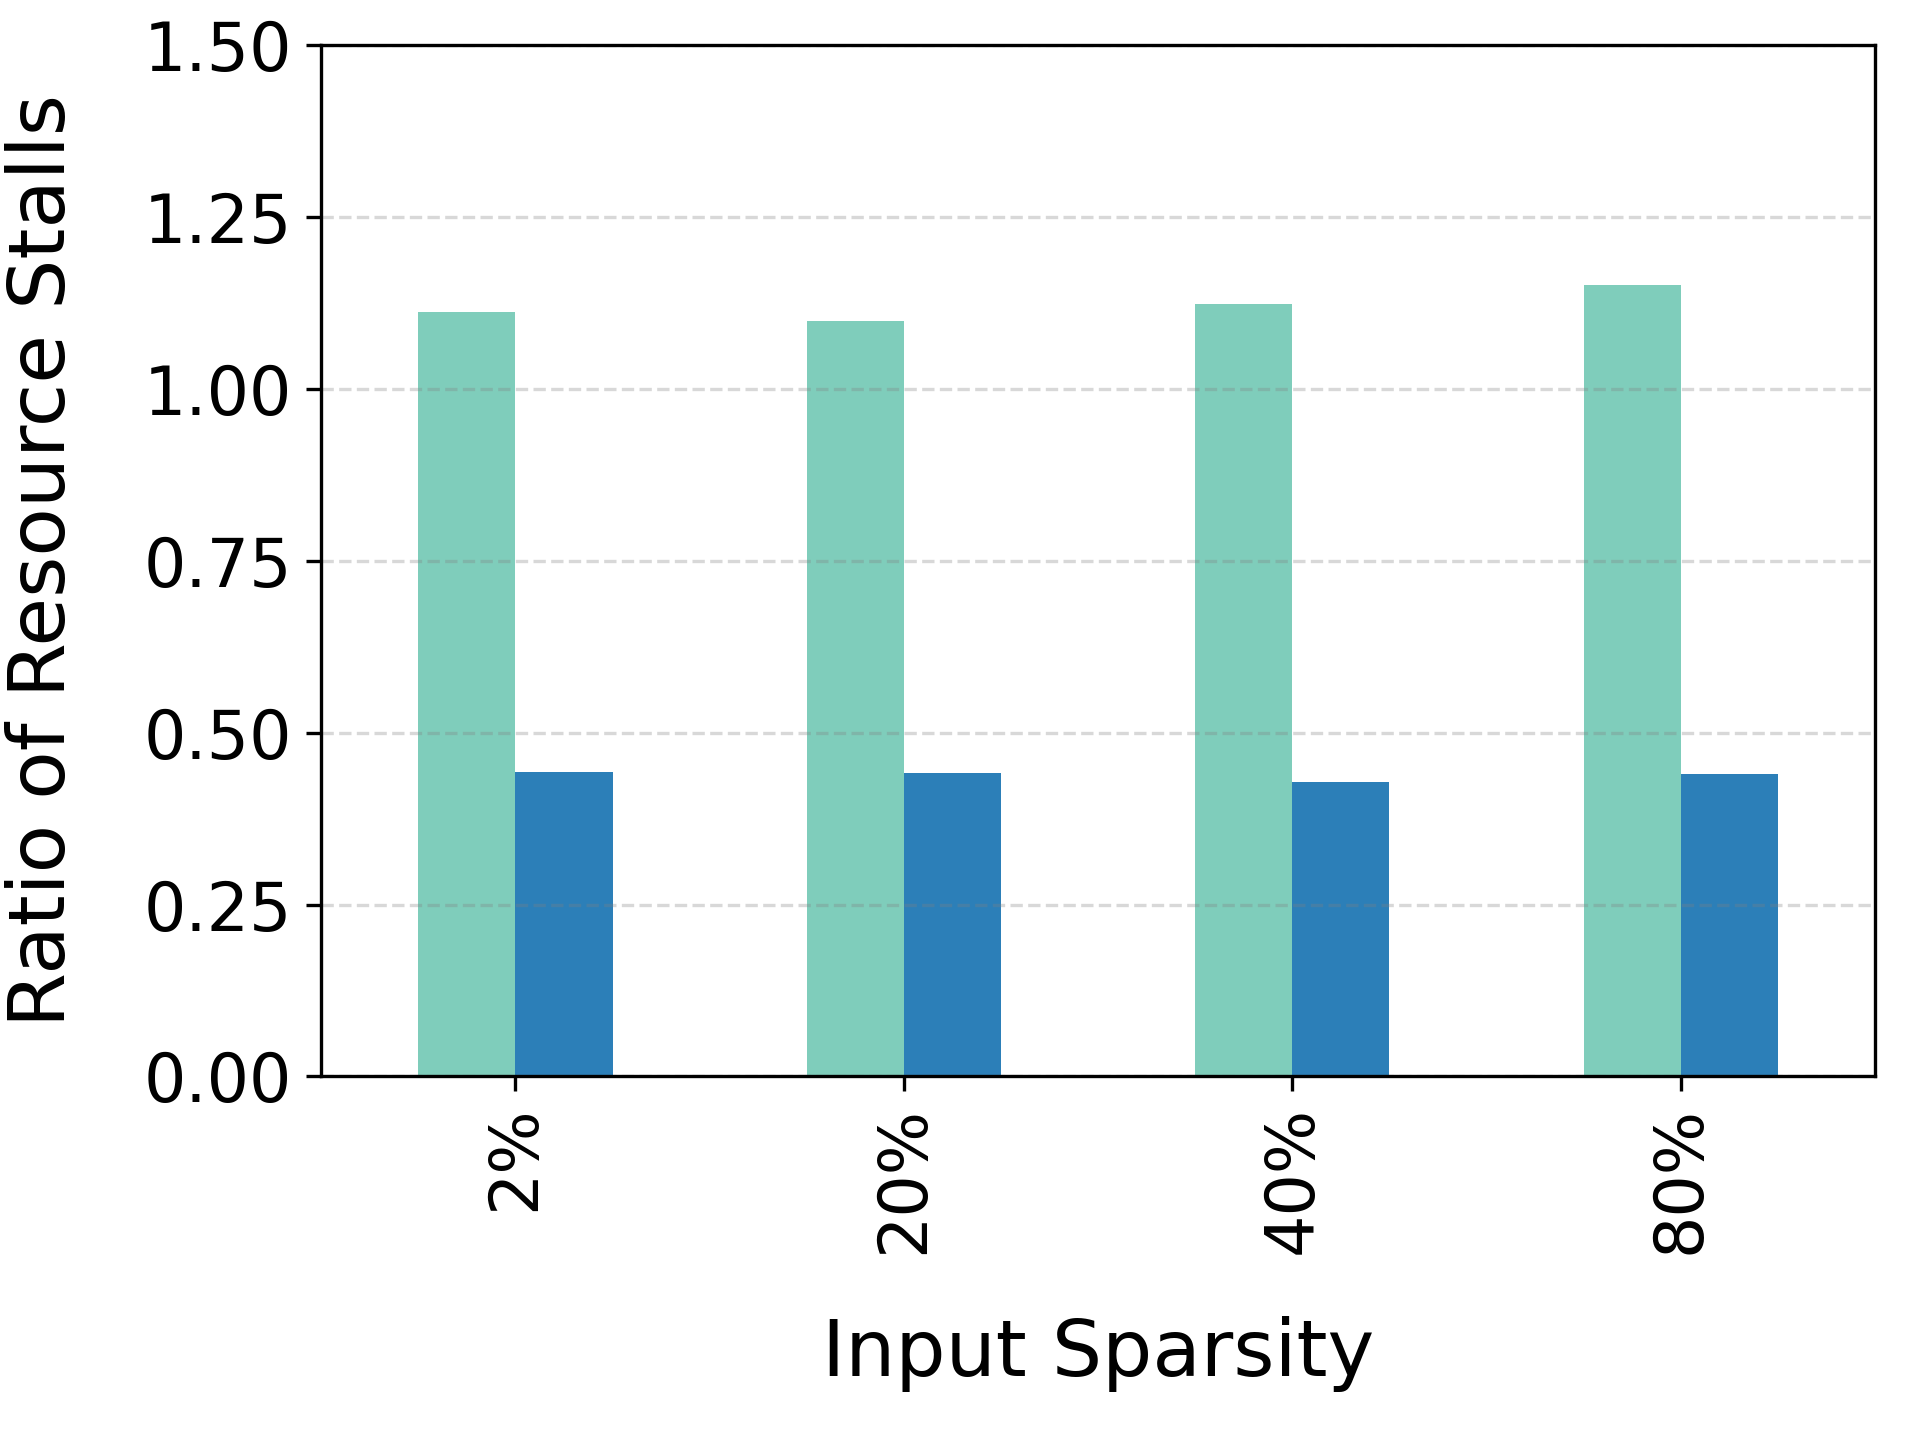
\includegraphics[width=\textwidth, height=.28\textheight]{Figures/Evaluations/if_then_else_few_scatter_resource_stalls.png}
    \caption{Ratio of resource-busy-induced stalls.}
    \label{fig:if-then-else-few-scatter-resource-stalls}
  \end{subfigure}%
  \begin{subfigure}{.5\textwidth}
        \centering
    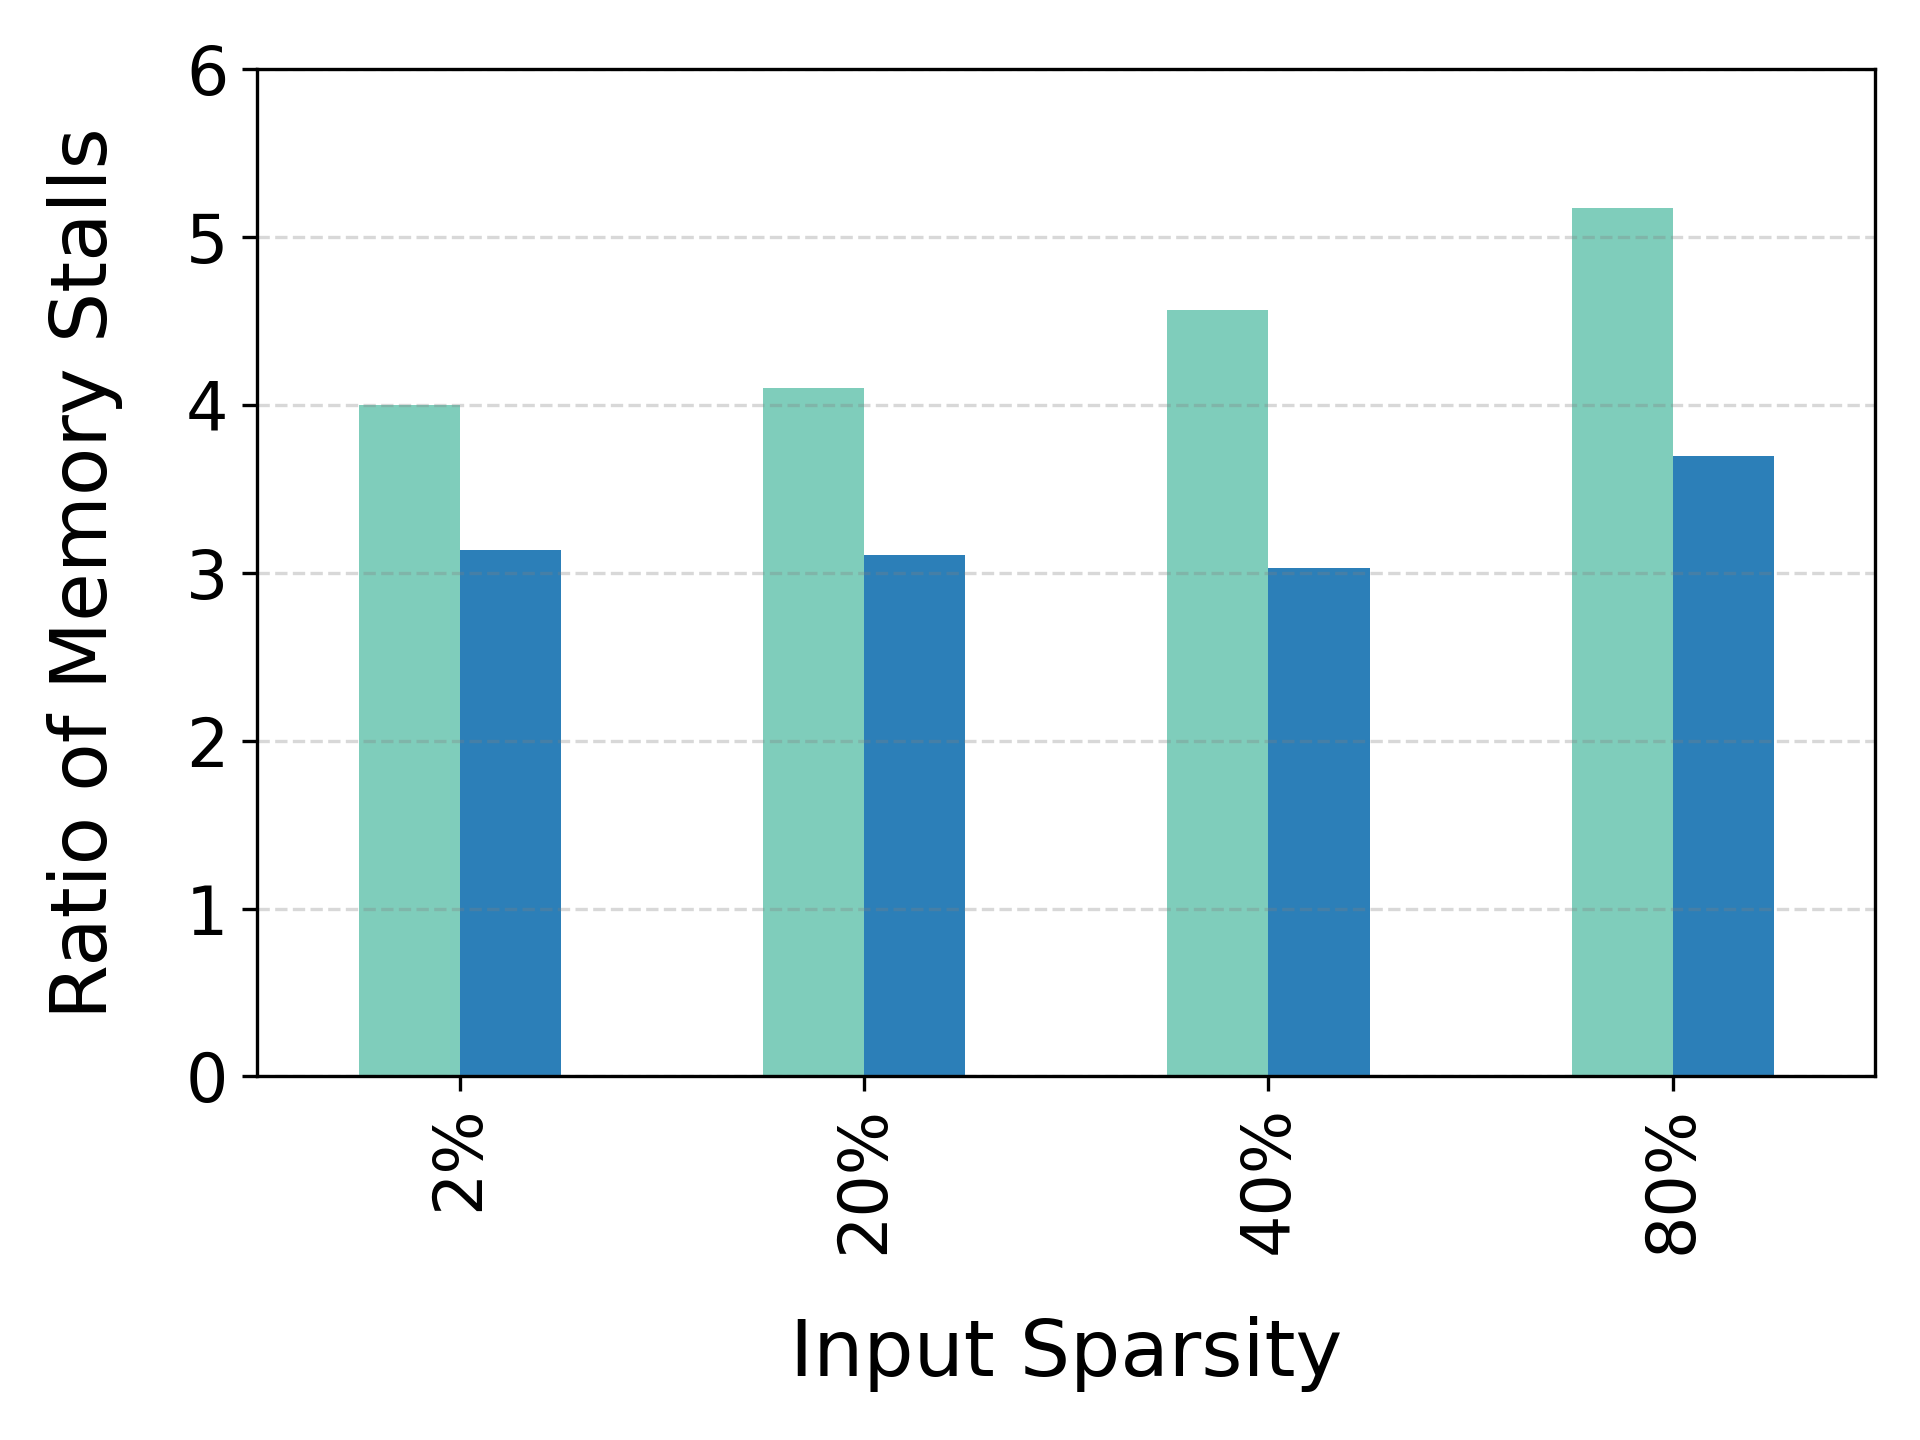
\includegraphics[width=\textwidth, height=.28\textheight]{Figures/Evaluations/if_then_else_few_scatter_mem_stalls.png}
    \caption{Ratio of memory-induced stalls.}
    \label{fig:if-then-else-few-scatter-mem-stalls}
  \end{subfigure}%
  \caption{Evaluation of the \ifElseBench micro-benchmark modified to have fewer store instructions. All metrics are normalized with respect to \ifconverted code (\ifconv).}
\end{figure*}


\begin{figure*}[h!]
  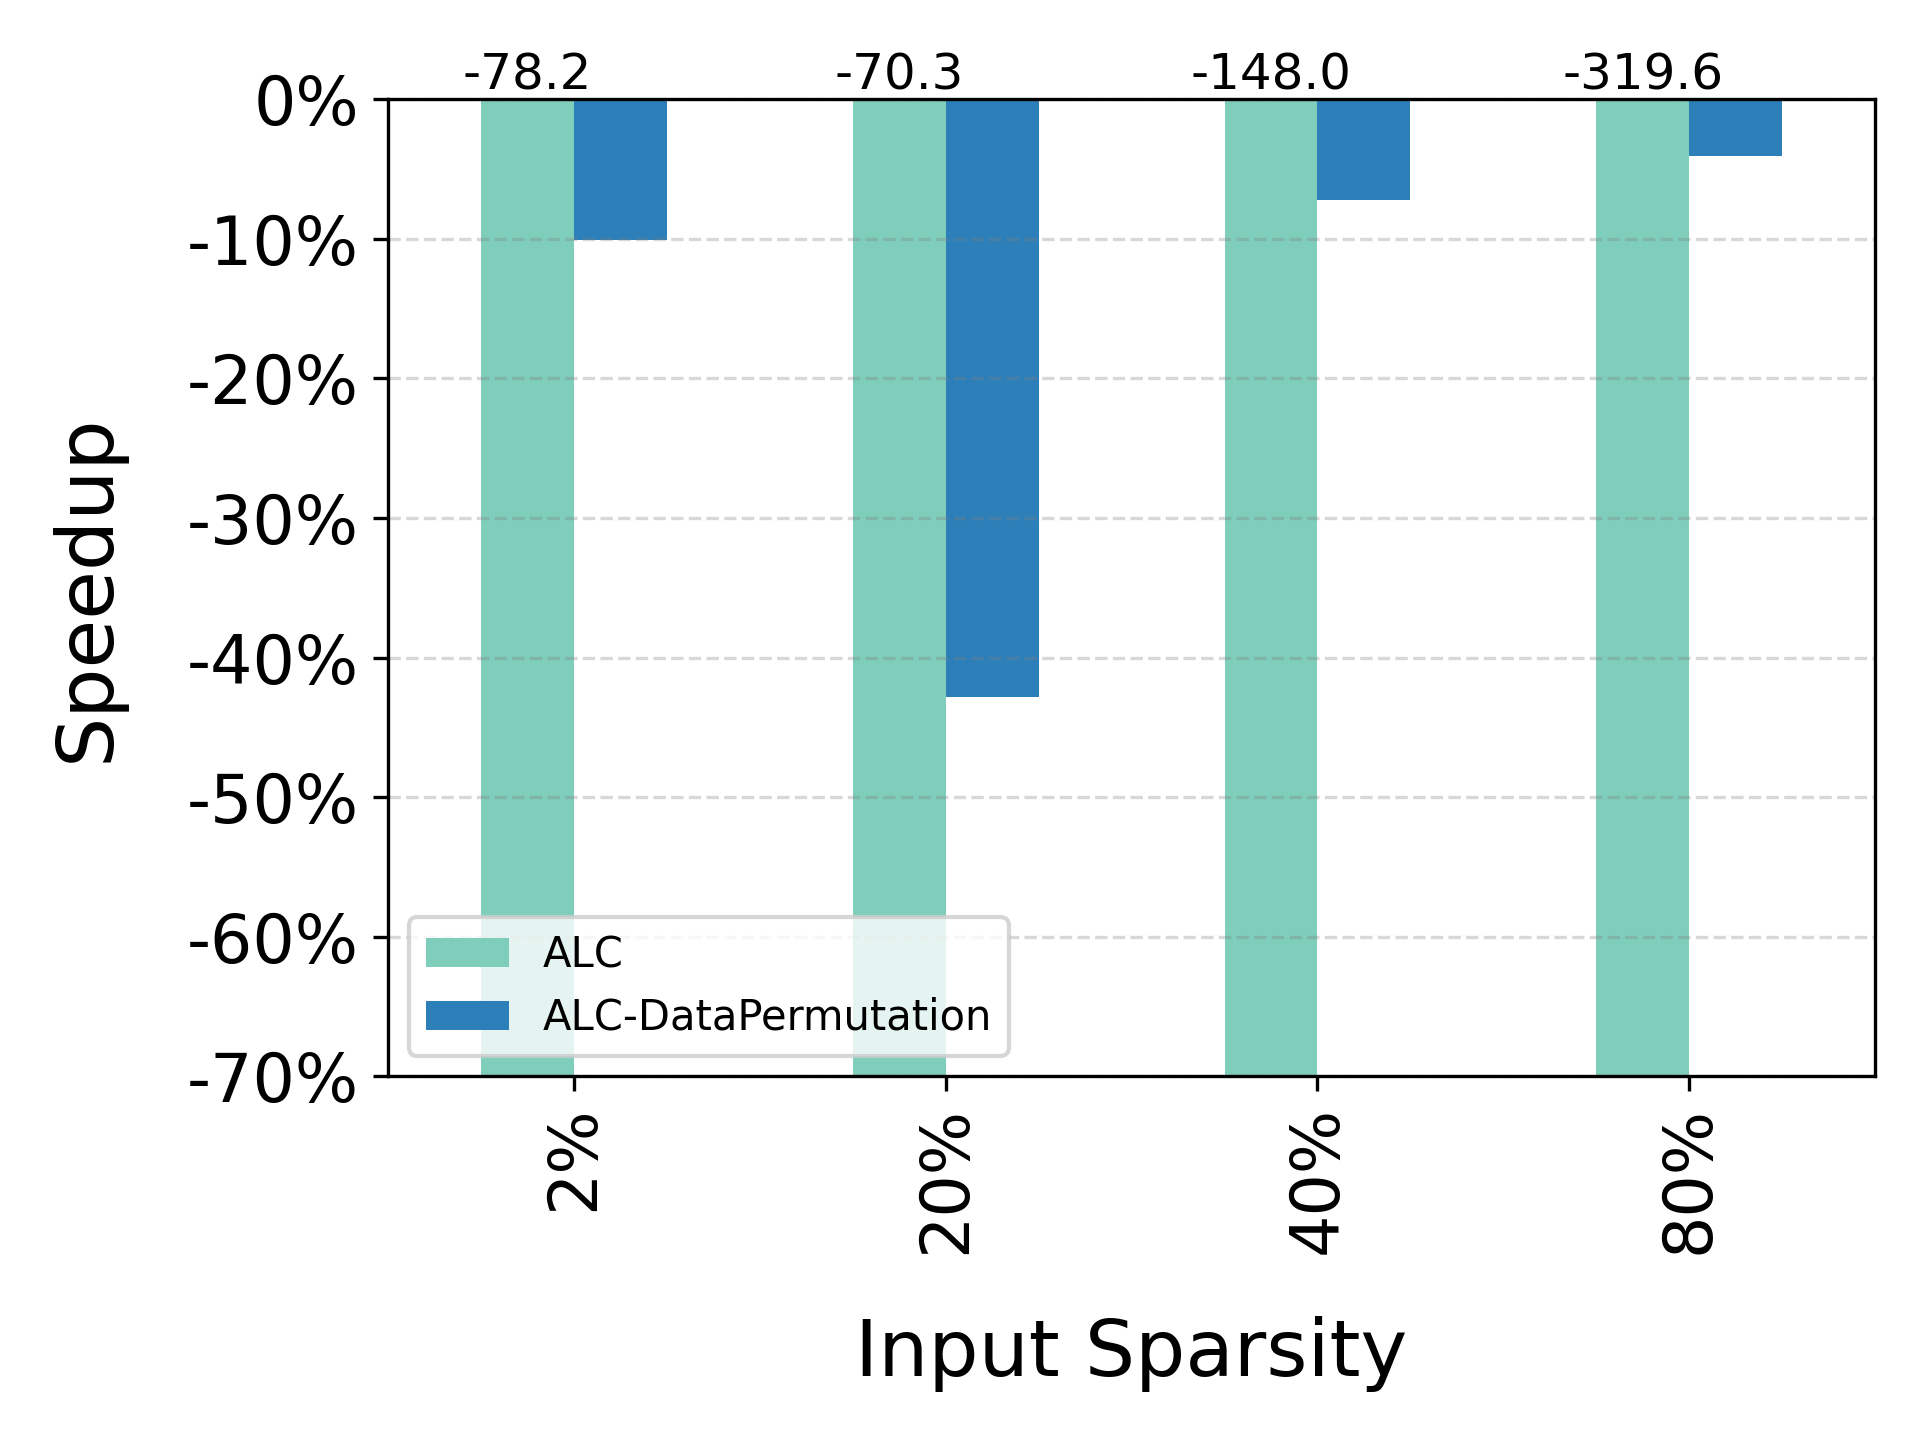
\includegraphics[width=0.8\textwidth]{Figures/Evaluations/single_if_many_scatter_speedup.png}
  \caption{ALC and Data Permutation speedups over If-Conversion for \ifThenBench micro-benchmark that has only one CFDPs.}
  \label{fig:single-if-many-scatter-speedup}
\end{figure*}

In this experiment, the code of the \ifElseBench micro-benchmark is modified to have fewer stores --- only one per \cpath ---, but it has the same number of arithmetic and load operations.
Fewer store operations translate to fewer scatter instructions in the compiler-generated ALC code.
Therefore, an increase in ALC's performance with fewer scatter operations indicates a positive answer to \circled{2}.

As \rfig{if-then-else-few-scatter-speedup} indicates, with fewer scatter stores both \ALC and \ALCdp outperform the baseline \ifconv.
Moreover, \ALCdp is four times faster than \ALC, outperforming \ifconv by up to $79\%$ in the $2\%$ sparsity case, a strong indicator of the effectiveness of eliminating both predicated instructions and gather loads.

\rfig{if-then-else-few-scatter-inst} shows the ratio of instructions executed, normalized to \ifconv. Similar to the previous case, \ALCdp executes considerably more instructions compared to \ALC which is due to the many instructions used for permuting data. An interesting observation is that, unlike \rfig{if-then-else-many-scatter-inst} where \ALC was executing almost the same amount of instructions as \ifconv, in this case, and especially in more sparse inputs, it has executed fewer instructions compared to \ifconv.
As the number of instructions of \ALC gets closer to that if \ifconv, their performance gets closer to each other. The correlation between these two charts and the fact that \ALCdp outperforms both \ALC and \ifconv suggests that, in the absence of expensive memory instruction such as scatter store, a key factor for better performance is the number of dynamically executed instructions.

\rfig{if-then-else-few-scatter-resource-stalls} shows a significant reduction in the number of resource stalls for \ALCdp as a direct result of having fewer scatter store instructions and thus explains the speedup over \ifconv.
Stalls due to memory operations follow the same trend as in the \ifElseBench micro-benchmark, as indicated in \rfig{if-then-else-few-scatter-mem-stalls}, evidence that arithmetic operations can amortize the effects of memory stalls.
Still, address calculations for gather/scatter instructions compete for resources resulting in a significant number of resource-busy stalls. 



\begin{figure*}[h!]
  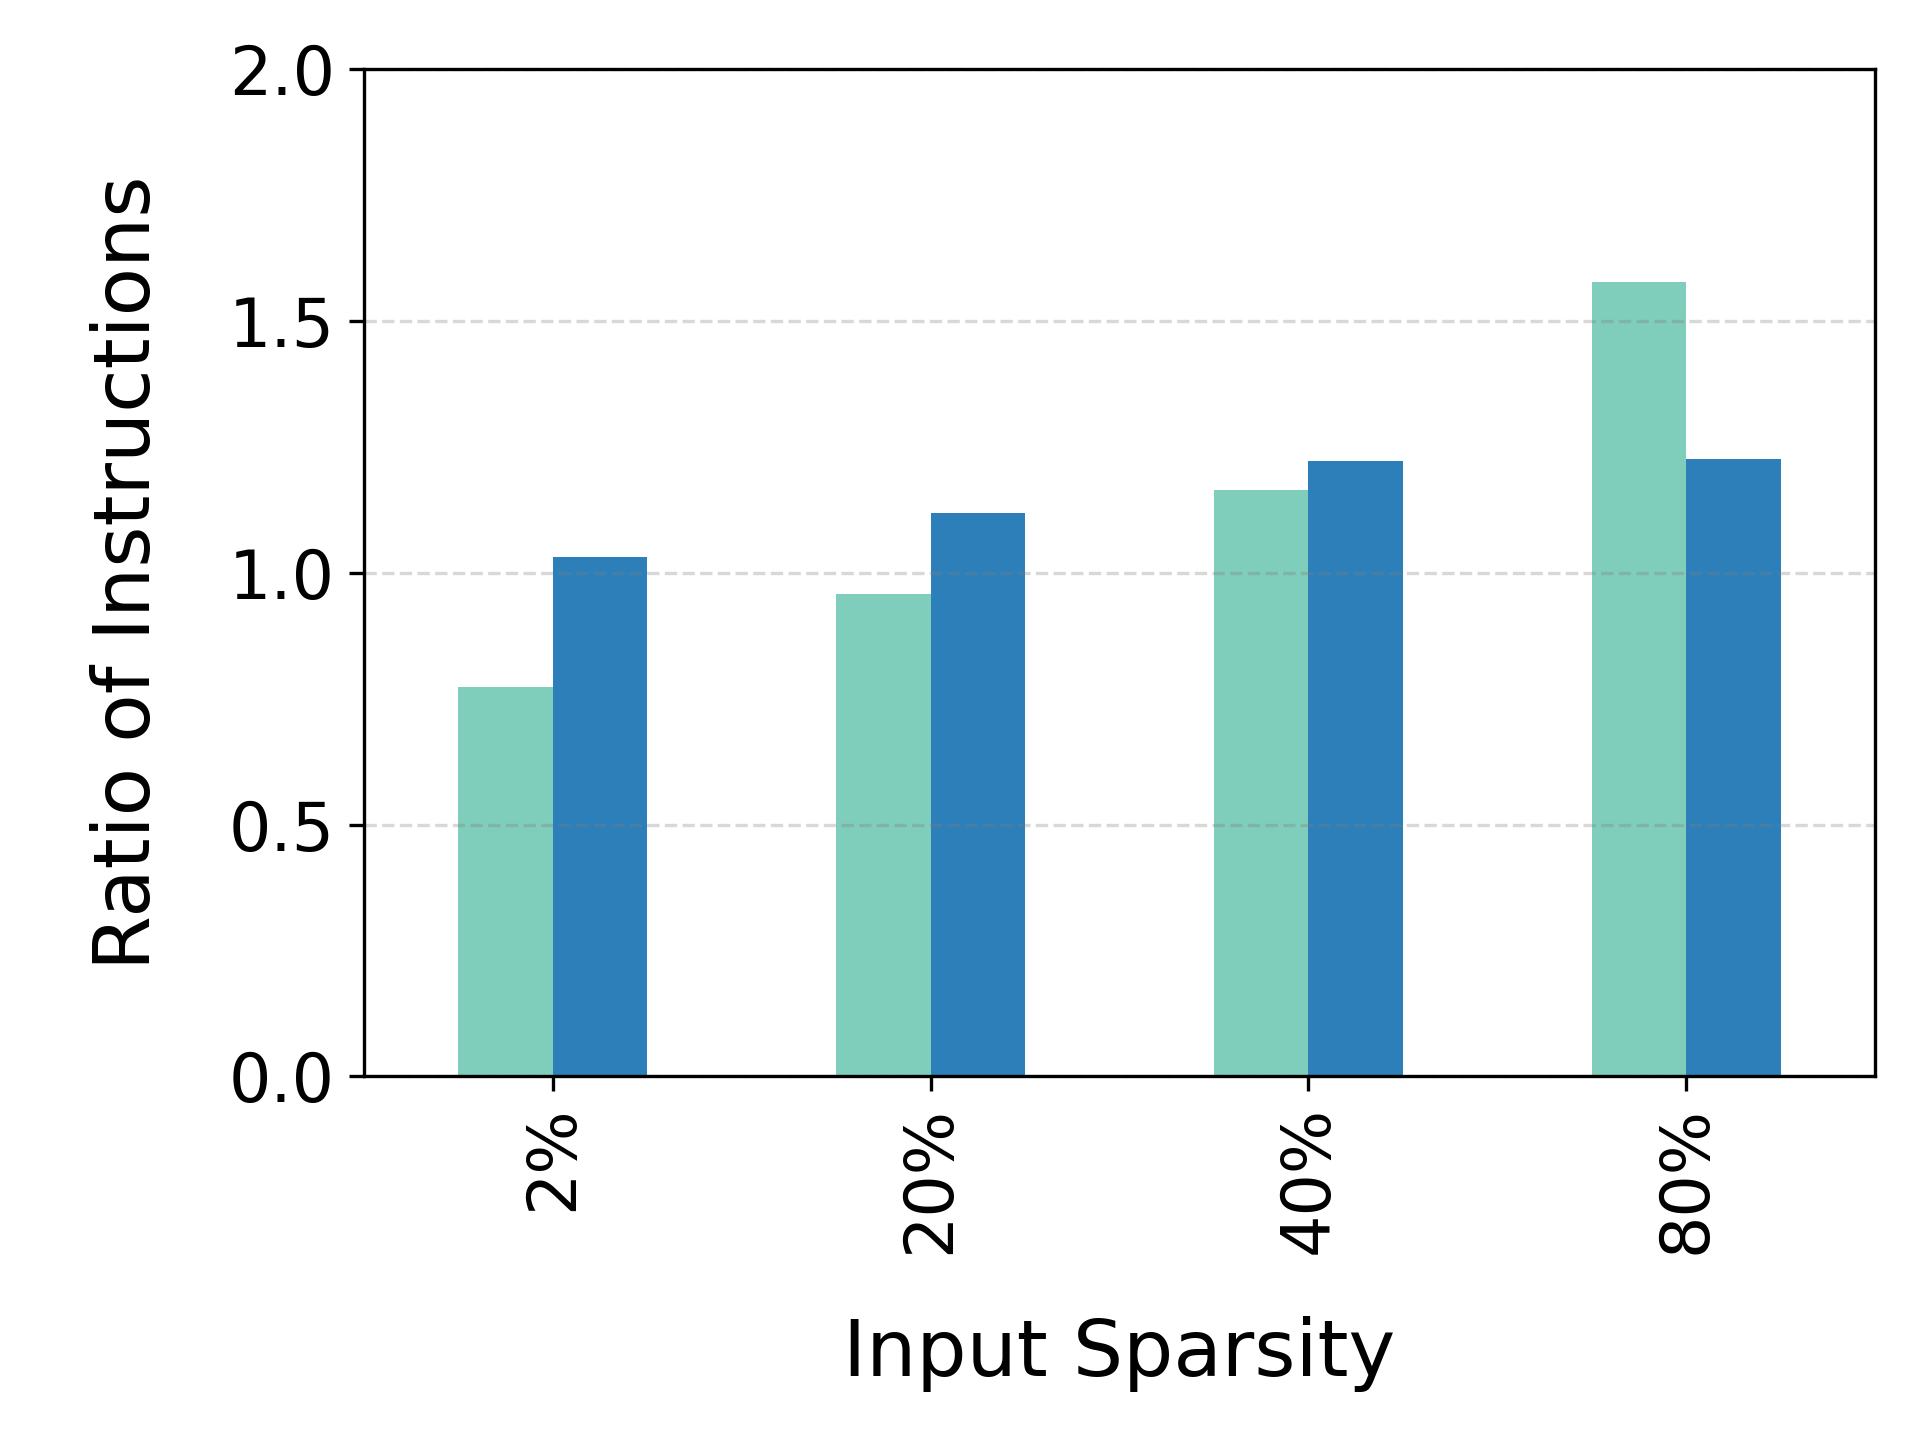
\includegraphics[width=0.8\textwidth]{Figures/Evaluations/single_if_many_scatter_instr.png}
  \caption{Ratio of dynamically executed instructions}
  \label{fig:single-if-many-scatter-inst}
\end{figure*}

\begin{figure*}[h!]
  \centering
 \begin{subfigure}{4cm}
    \centering
    
\includegraphics[width=\textwidth]{Figures/Evaluations/Legend.png}
 \end{subfigure}\\
  \begin{subfigure}{.5\textwidth}
    \centering
    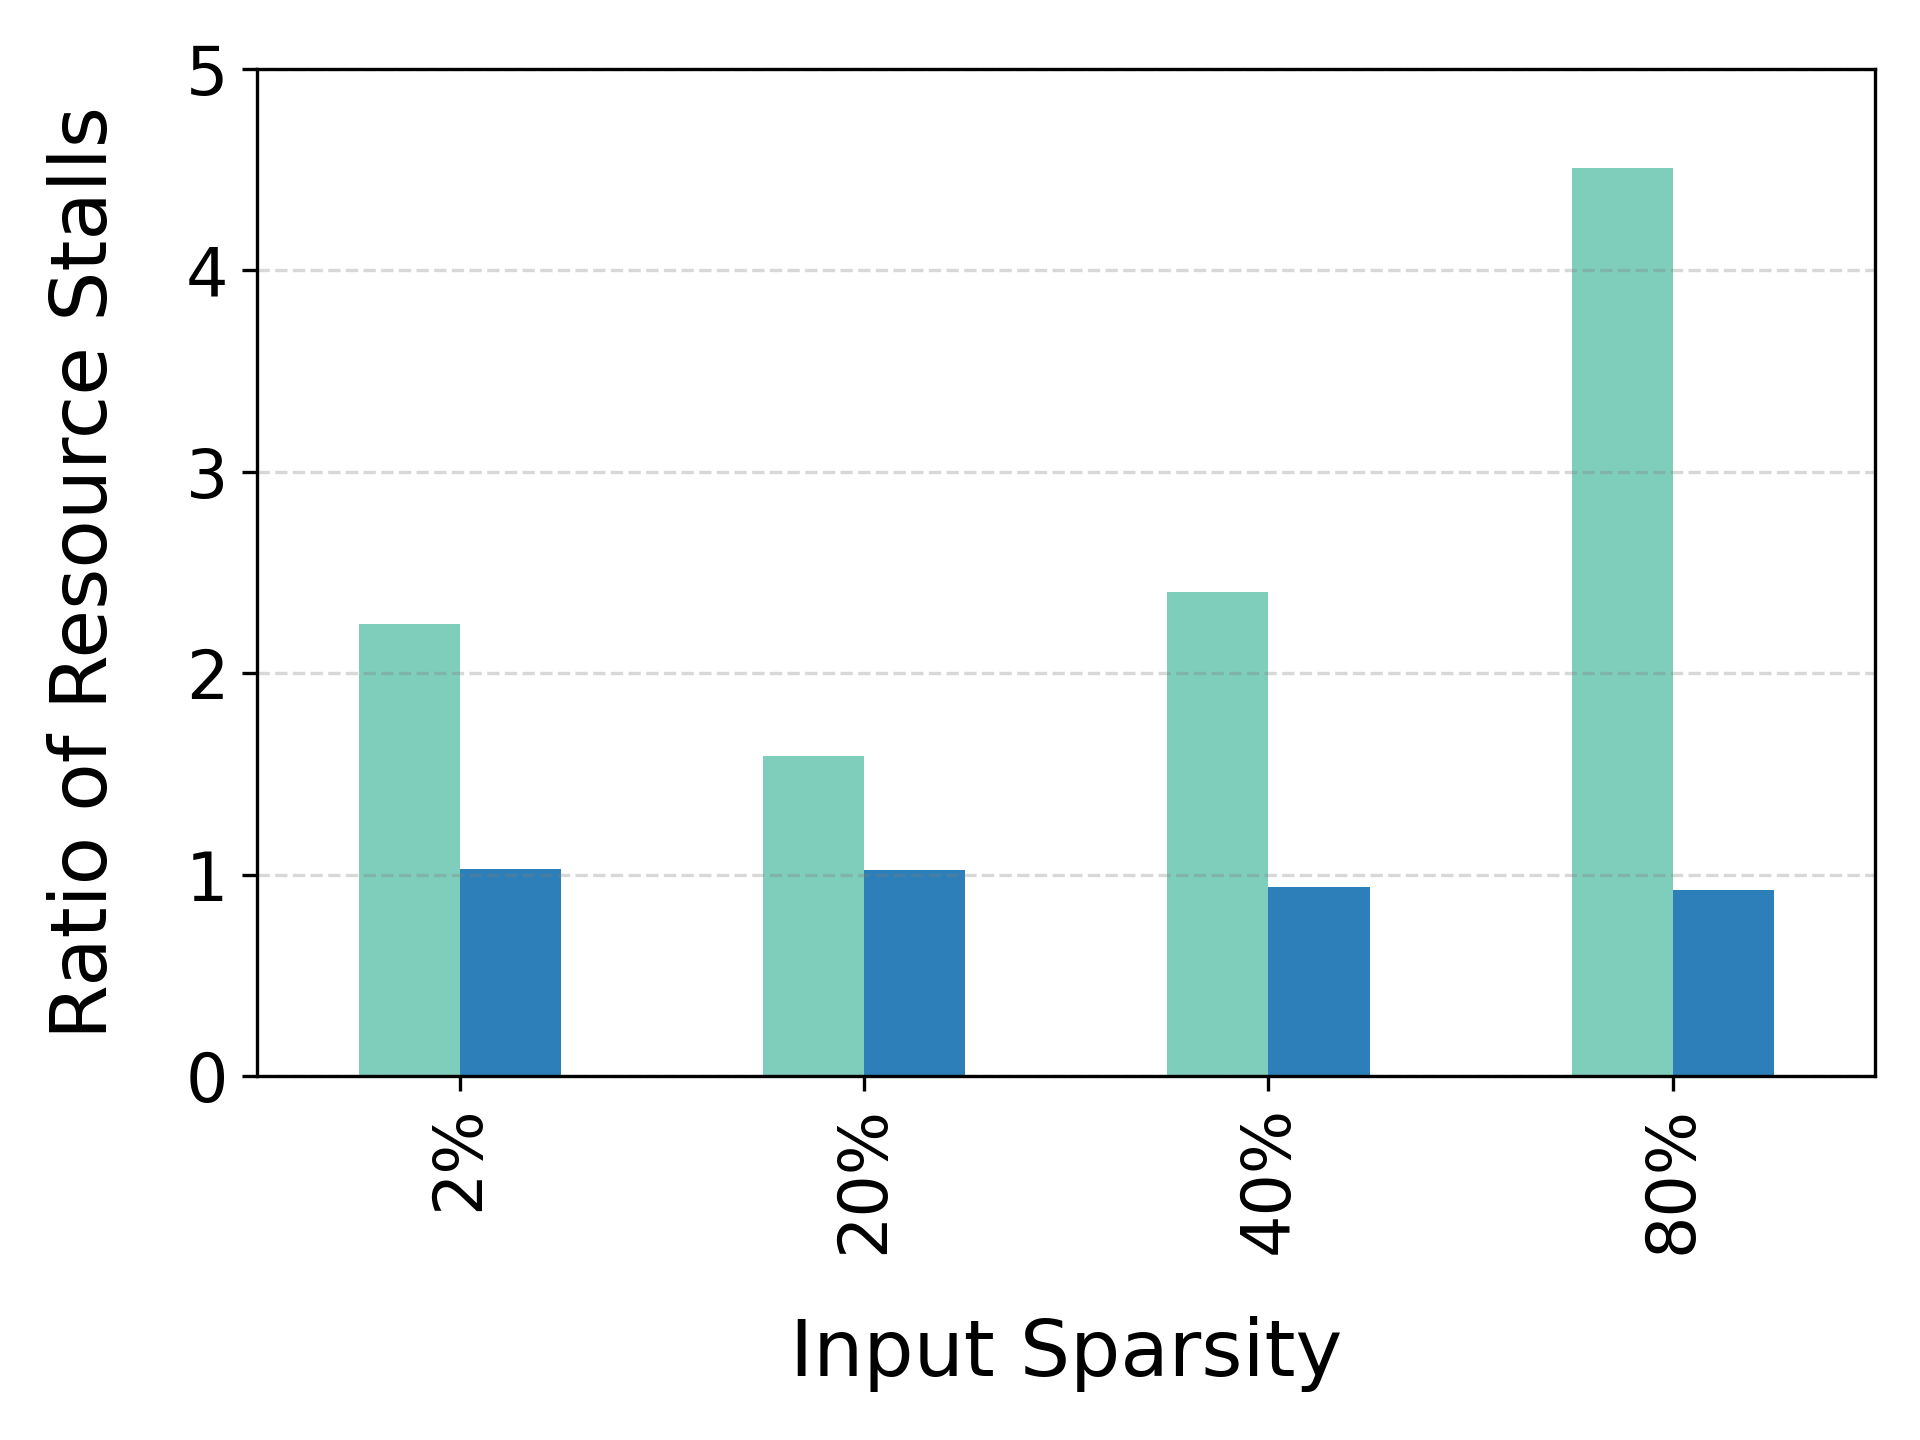
\includegraphics[width=\textwidth, height=.28\textheight]{Figures/Evaluations/single_if_many_scatter_resource_stalls.png}
    \caption{Ratio of resource-busy-induced stalls.}
    \label{fig:single-if-many-scatter-resource-stalls}
  \end{subfigure}%
  \begin{subfigure}{.5\textwidth}
        \centering
    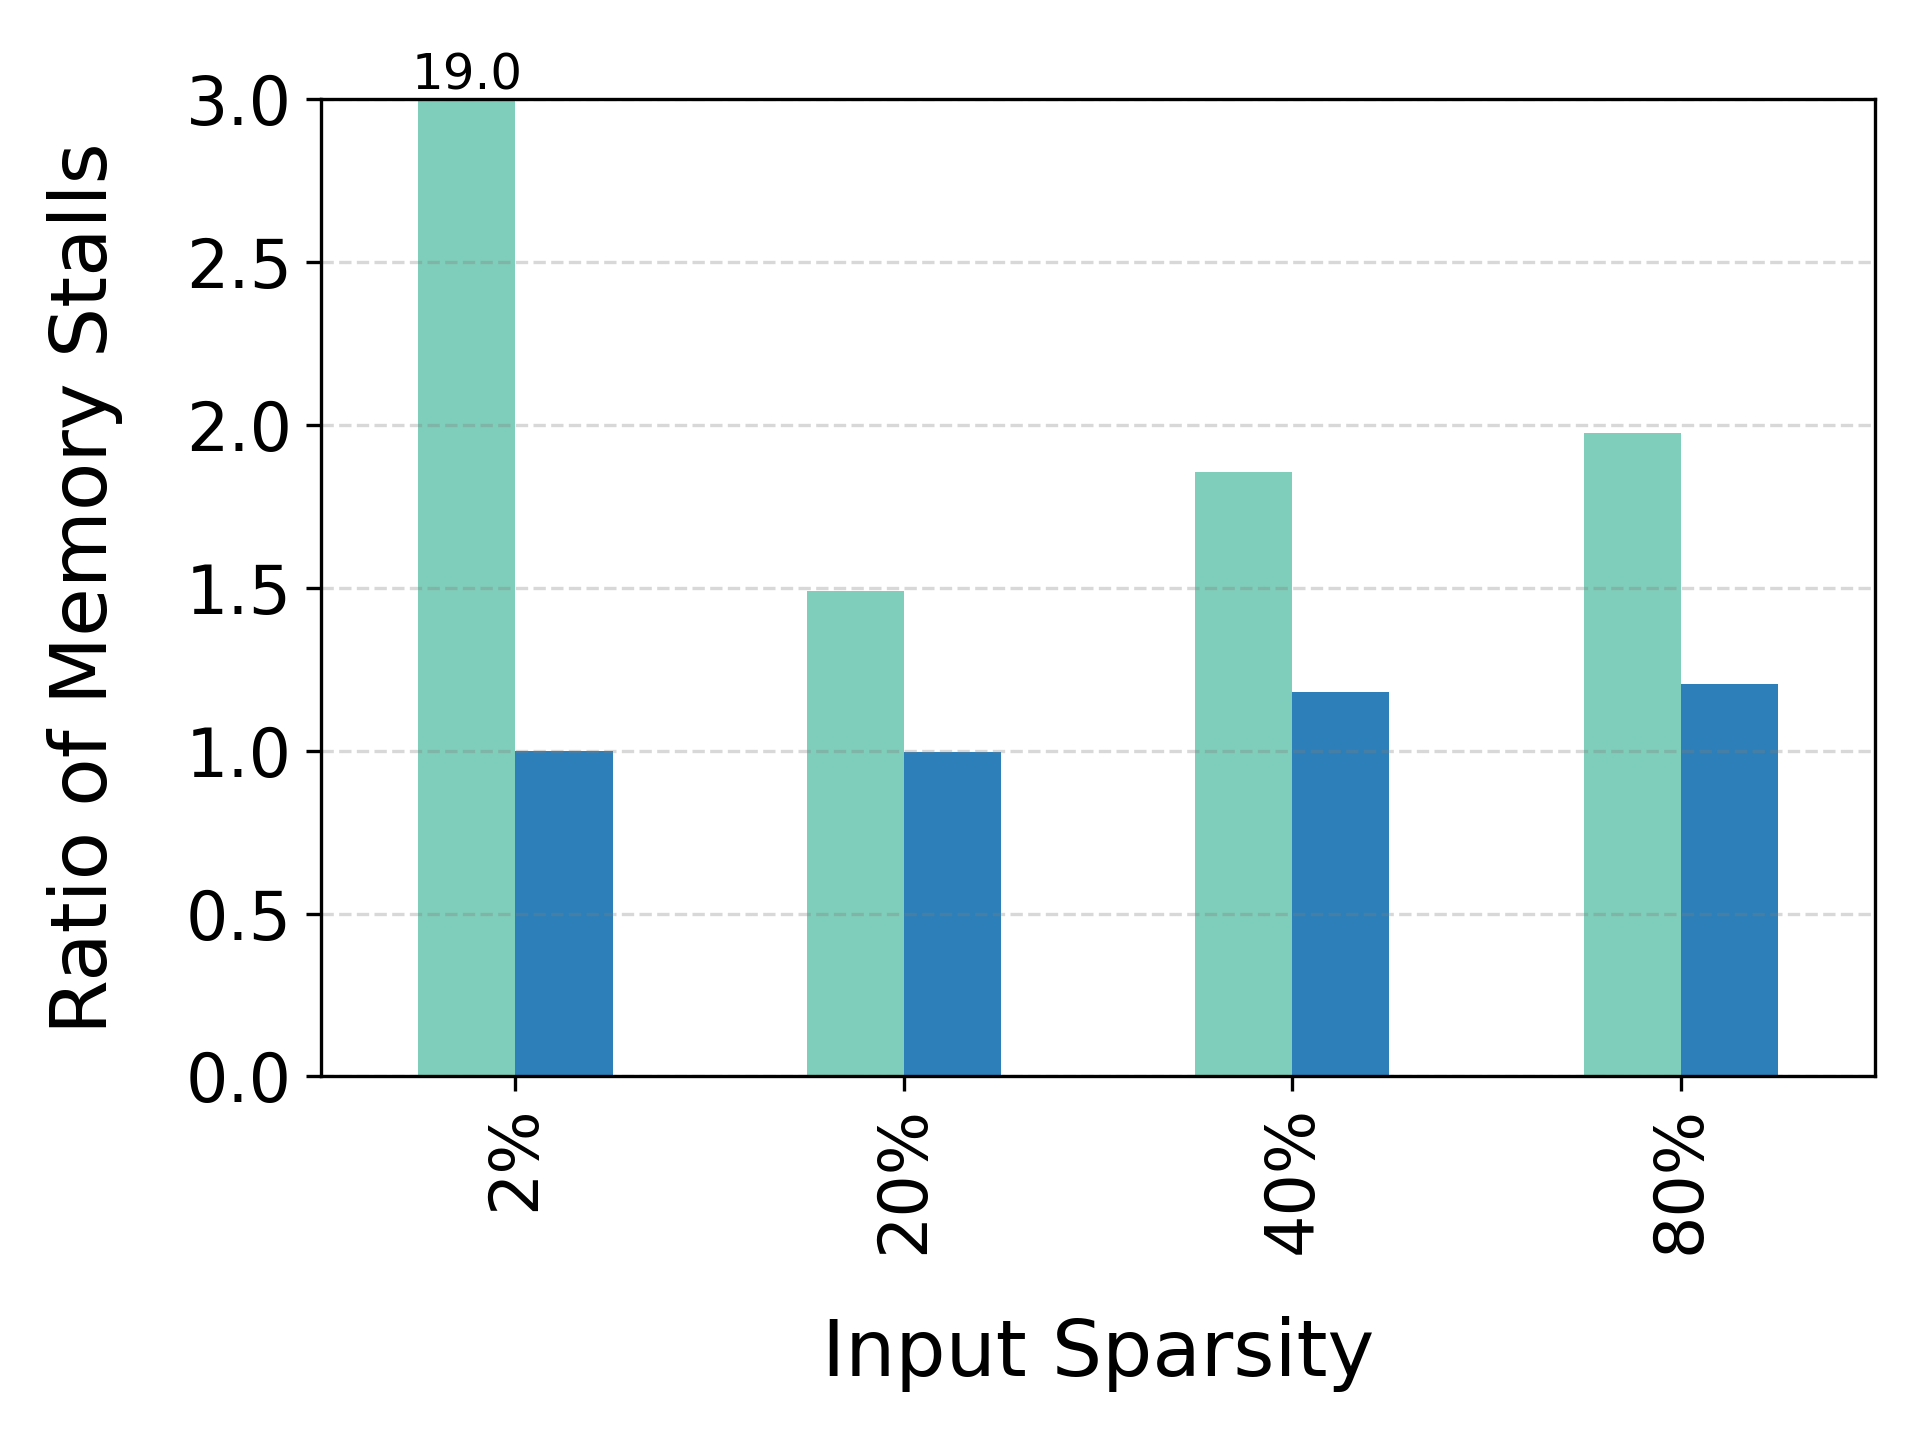
\includegraphics[width=\textwidth, height=.28\textheight]{Figures/Evaluations/single_if_many_scatter_mem_stalls.png}
    \caption{Ratio of memory-induced stalls.}
    \label{fig:single-if-many-scatter-mem-stalls}
  \end{subfigure}%
  \caption{Evaluation of the \ifElseBench micro-benchmark modified to have fewer store instructions. All metrics are normalized with respect to \ifconverted code (\ifconv).}
\end{figure*}

\section{Data Permutation Improves ALC}
\label{sec:eval-single-if}

This experiment evaluates the ALC algorithm modification discussed in \rsec{single-if-statement-approach} on the \ifThenBench micro-benchmark.
\rfig{single-if-many-scatter-speedup} presents speedups of \ALC and \ALCdp over \ifconv.
In this case, both ALC versions are unable to provide improvements over \ifconv and result in performance degradation.
The single control-flow data path case is challenging for any variant of ALC because, unlike the \ifElseBench case that has two \cpaths, considerably fewer instructions are executed with inactive lanes.
The results indicate a negative answer to \circled{3}, \ie, in general, it is not beneficial to apply ALC on loops with a single \cpath.
Nevertheless, \ALCdp provides significant speedup over \ALC by eliminating gather load instructions.

\rfig{single-if-many-scatter-inst} shows that like cases with two \cpath, \ALCdp executes more instructions compared to \ALC. The only exception is $80\%$ sparsity where \ALC is executing significantly more instructions than both \ALCdp and \ifconv. The reason is that, for this sparsity, \ALCdp executes if-converted code for most of the iterations based on the algorithm proposed in \rfig{single-if}. When most predicates are true, in each iteration of the loop \ALC processes vectors that are \emph{almost} uniform. As a result, it always needs to both do the permutation and execute the \Then block which results in poor performance and in a significant number of instructions being executed.   

Moreover, and similar to the two \cpath cases, both memory and resource stalls are lower with \ALCdp than with \ALC, as \rfig{single-if-many-scatter-mem-stalls} and \rfig{single-if-many-scatter-resource-stalls} indicate.

\begin{figure*}[t]
  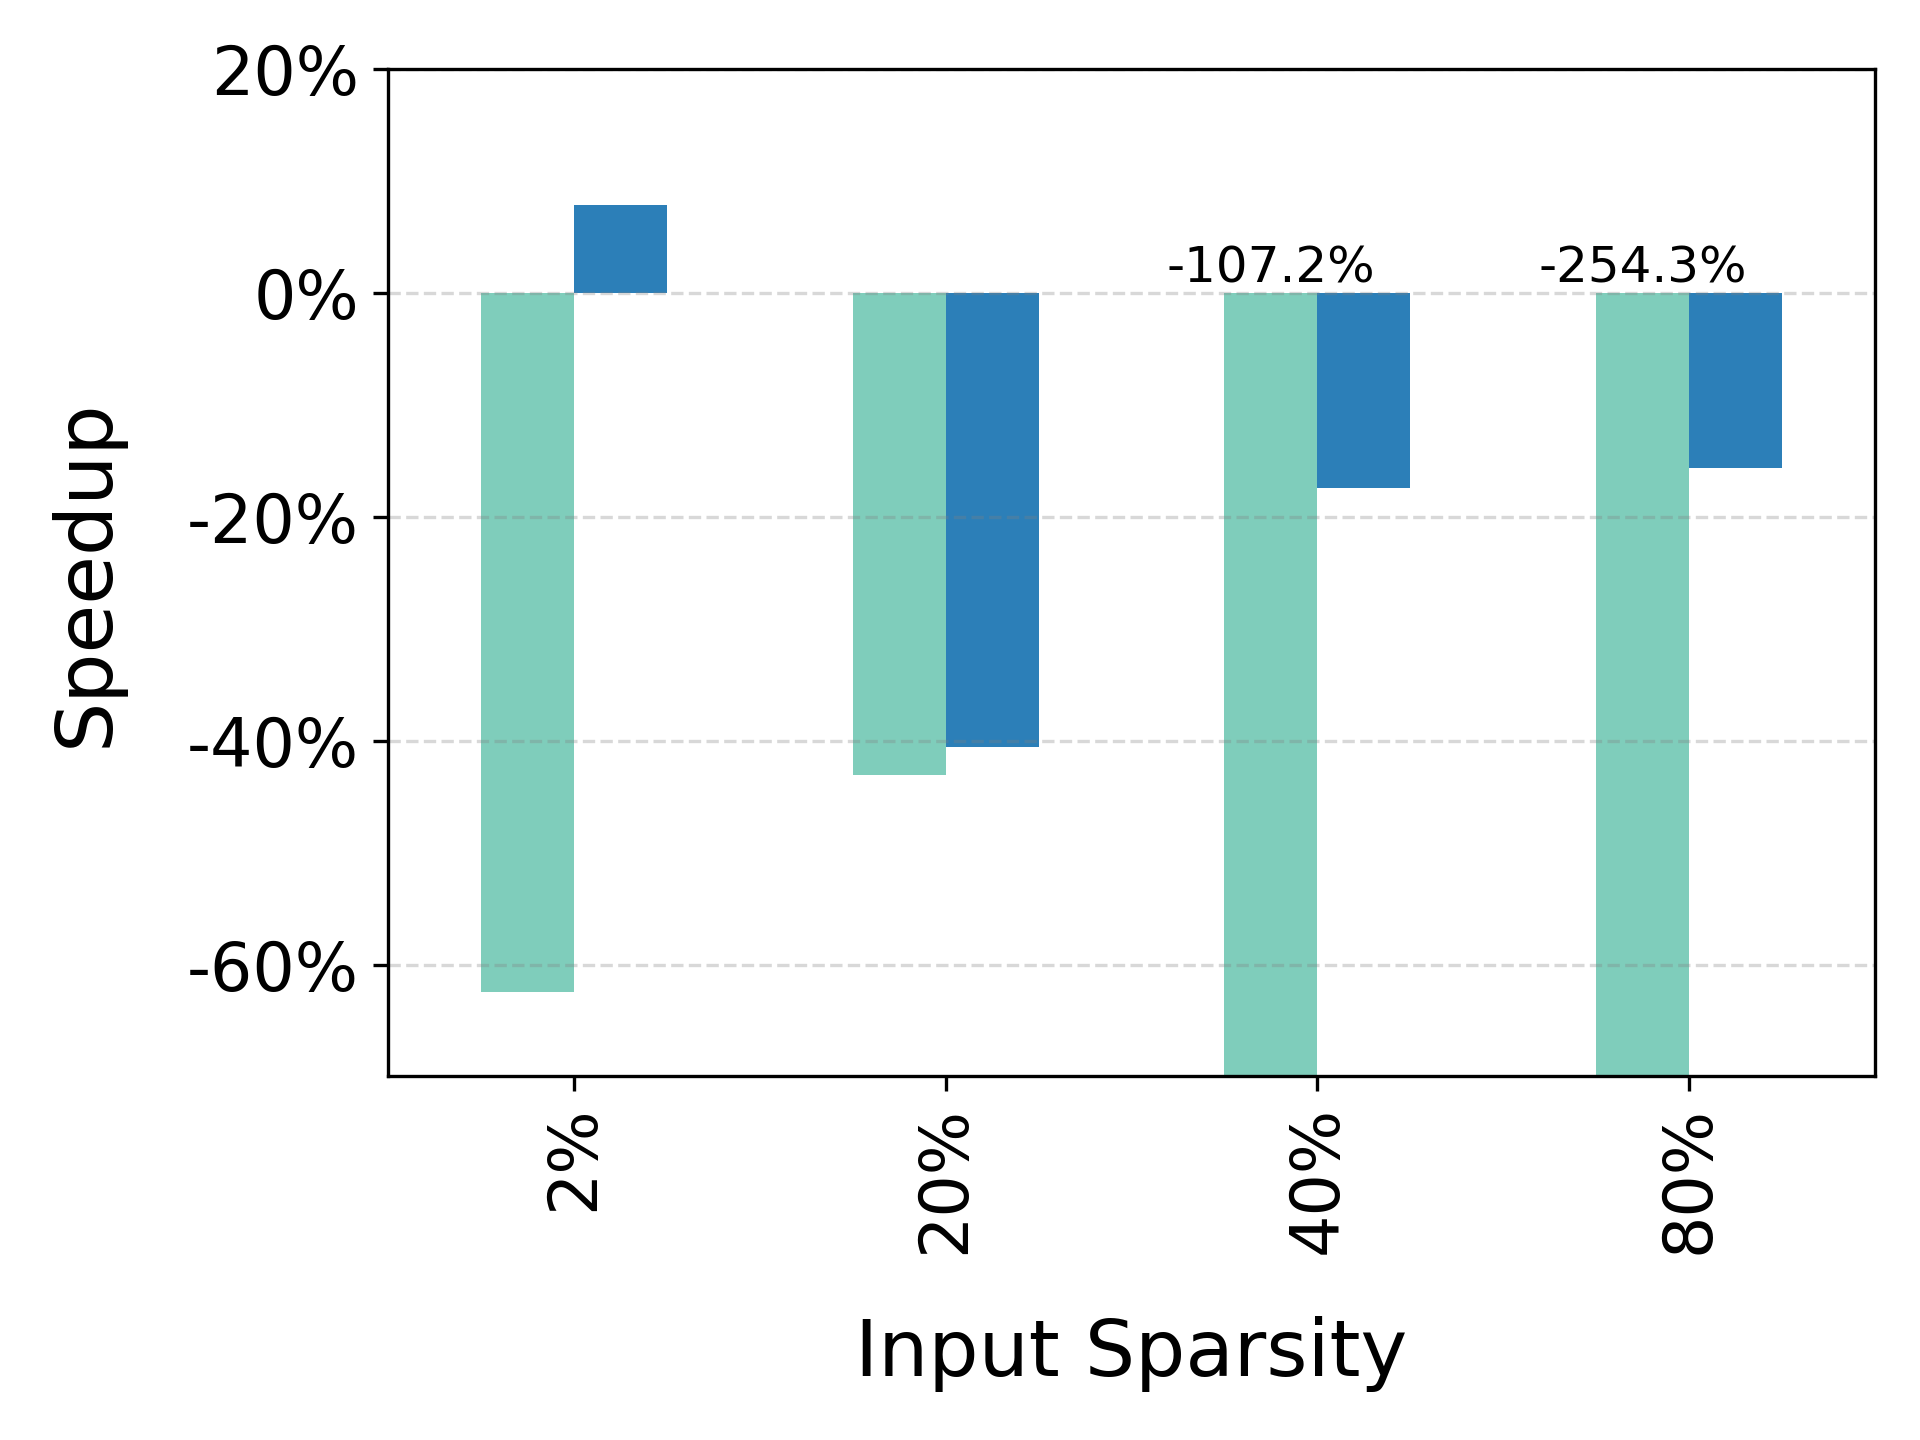
\includegraphics[width=0.8\textwidth]{Figures/Evaluations/single_if_few_scatter_speedup.png}
  \caption{Data Permutation and ALC Speedups in the presence of fewer Scatter instructions for \ifThenBench}
  \label{fig:single-if-few-scatter-speedup}
\end{figure*}

\begin{figure*}[h!]
  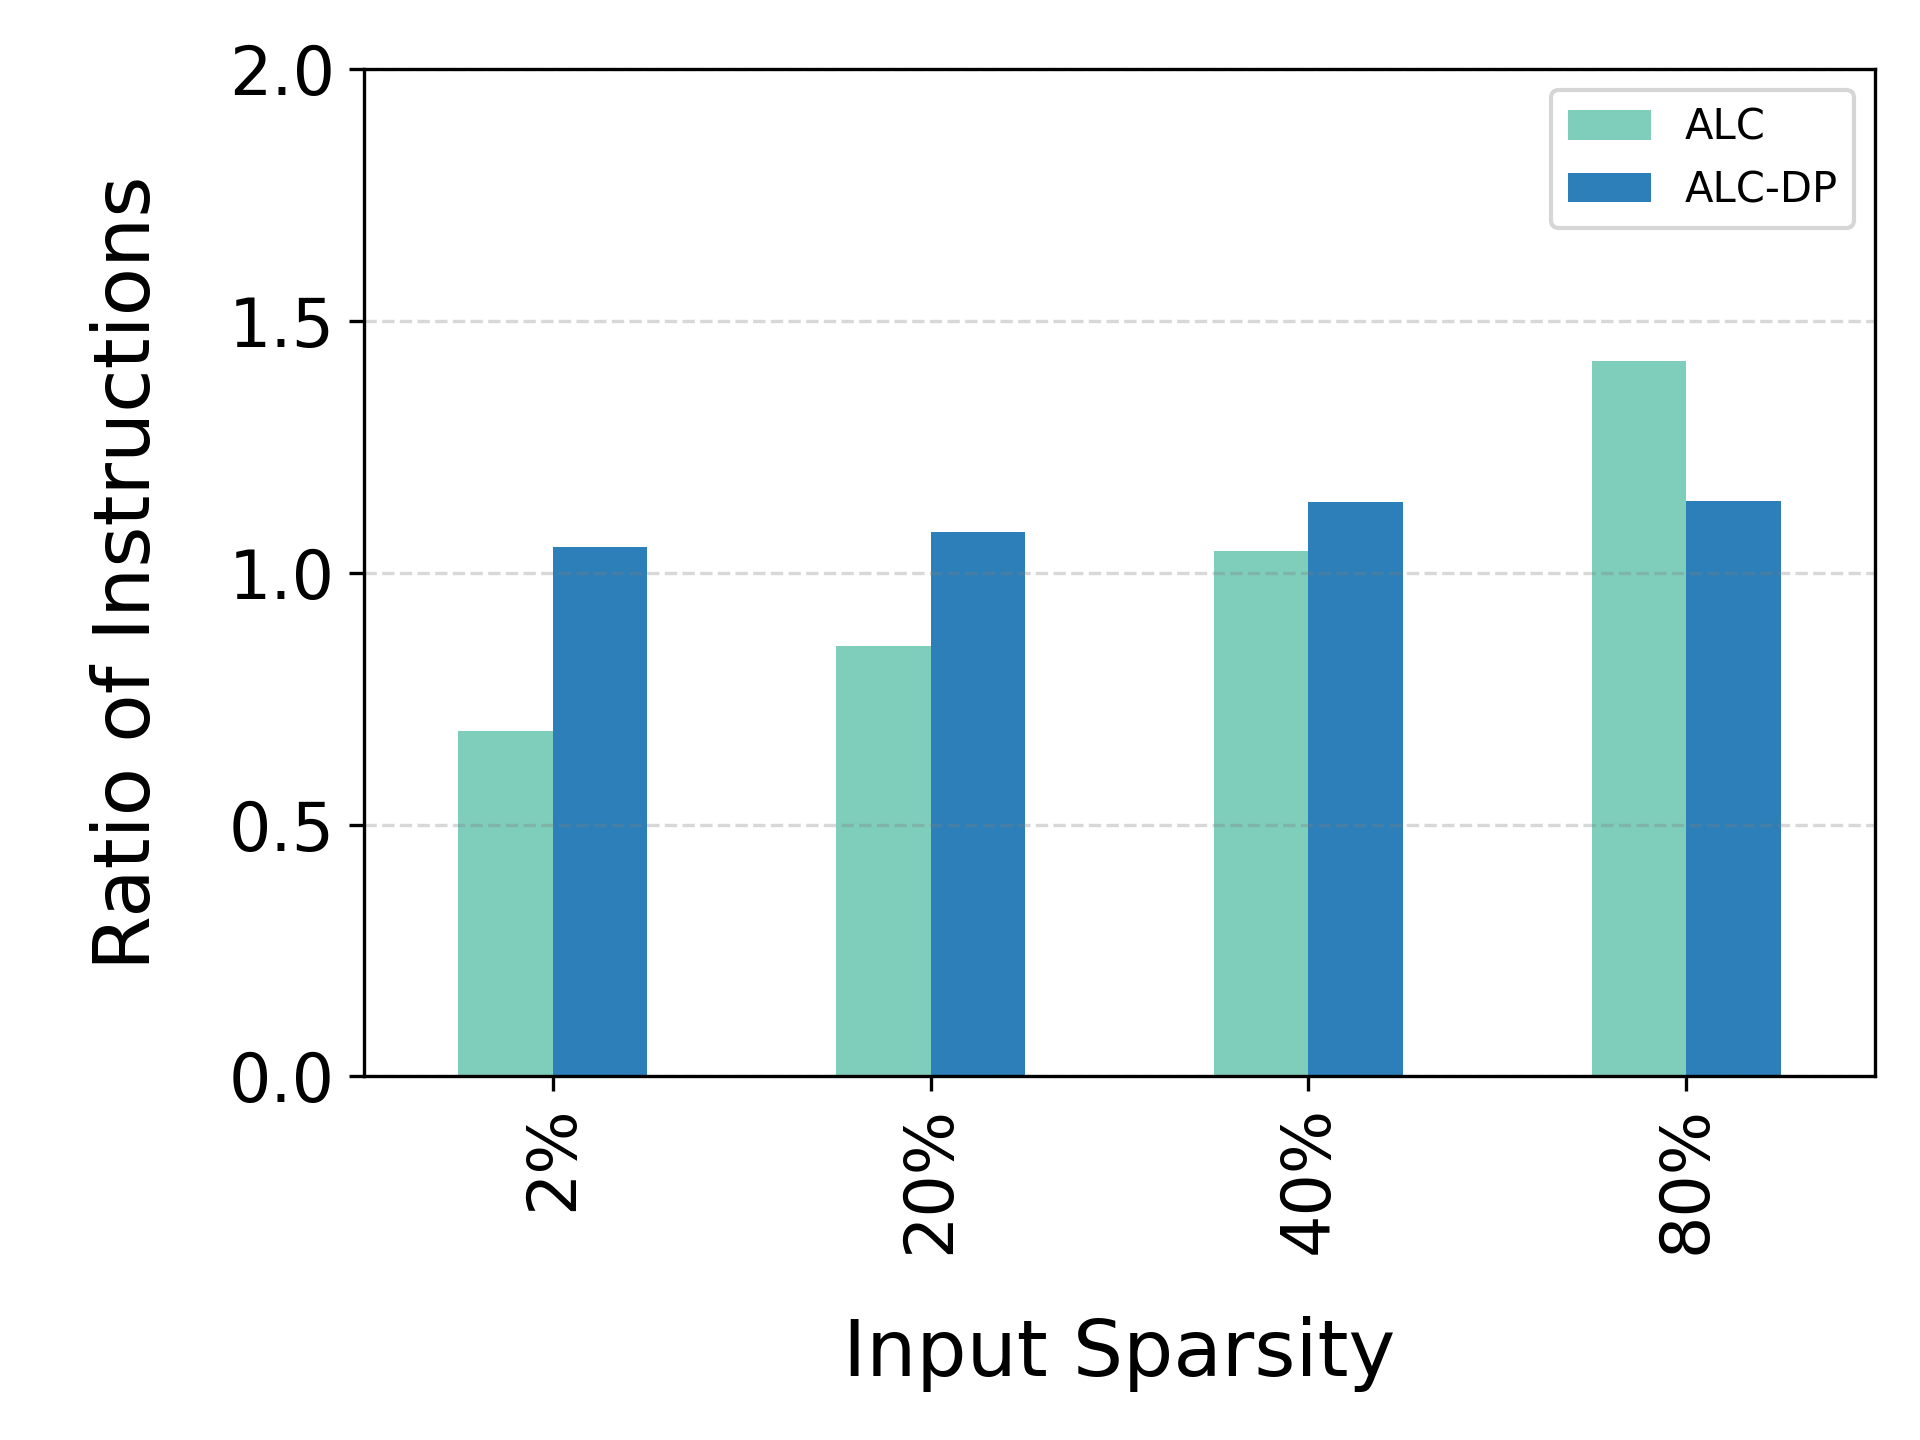
\includegraphics[width=0.8\textwidth]{Figures/Evaluations/single_if_few_scatter_instr.png}
  \caption{Ratio of dynamically executed instructions}
  \label{fig:single-if-few-scatter-inst}
\end{figure*}

\begin{figure*}[h!]
  \centering
 \begin{subfigure}{4cm}
    \centering
    
\includegraphics[width=\textwidth]{Figures/Evaluations/Legend.png}
 \end{subfigure}\\
  \begin{subfigure}{.5\textwidth}
    \centering
    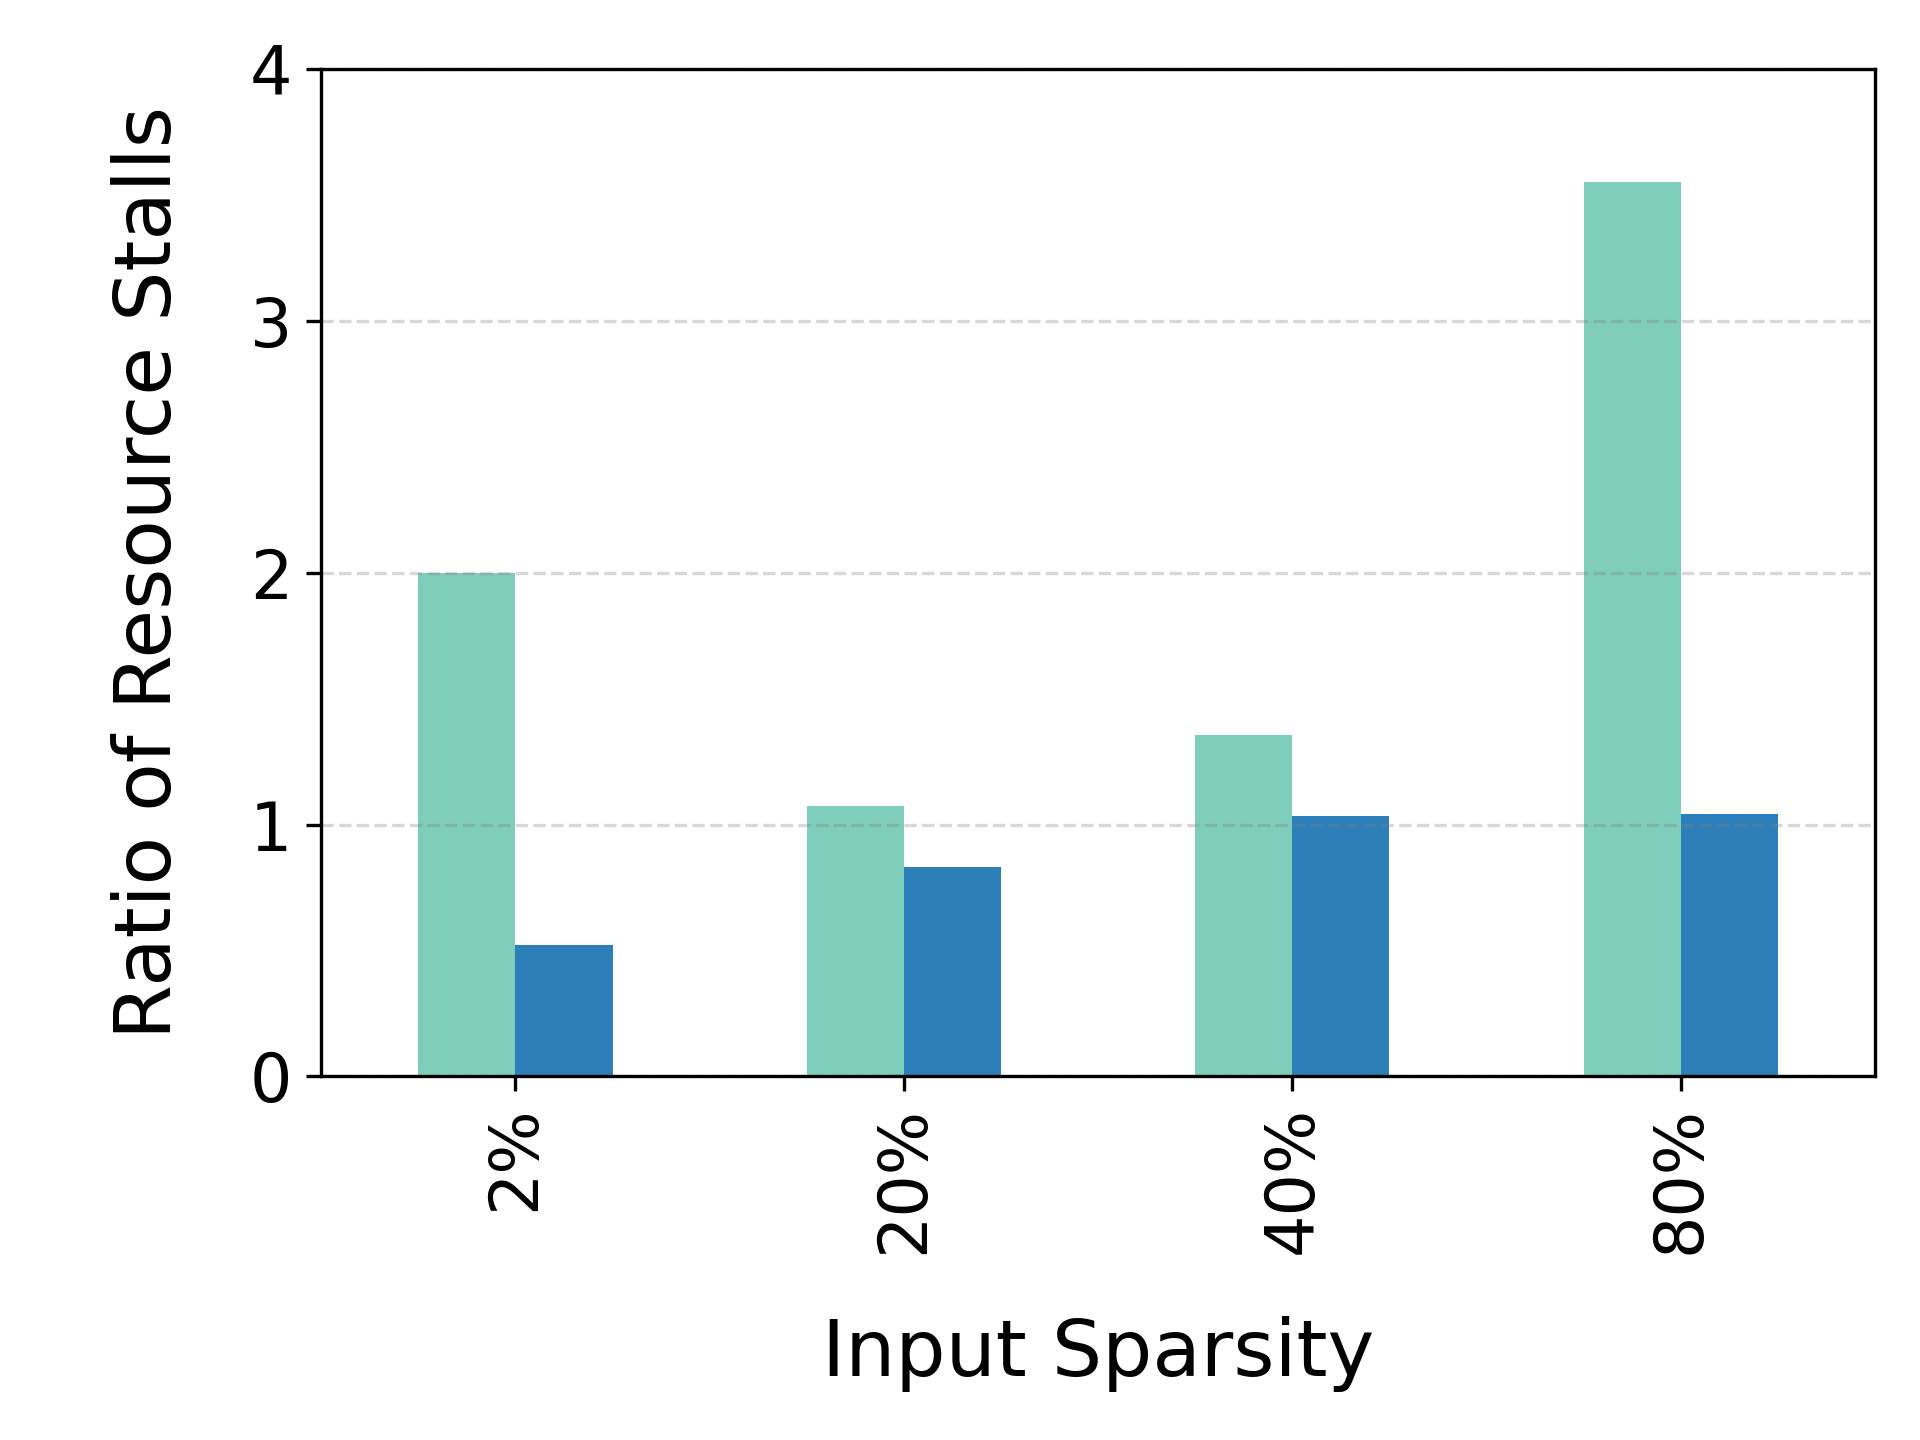
\includegraphics[width=\textwidth, height=.28\textheight]{Figures/Evaluations/single_if_few_scatter_resource_stalls.png}
    \caption{Ratio of resource-busy-induced stalls.}
    \label{fig:single-if-few-scatter-resource-stalls}
  \end{subfigure}%
  \begin{subfigure}{.5\textwidth}
        \centering
    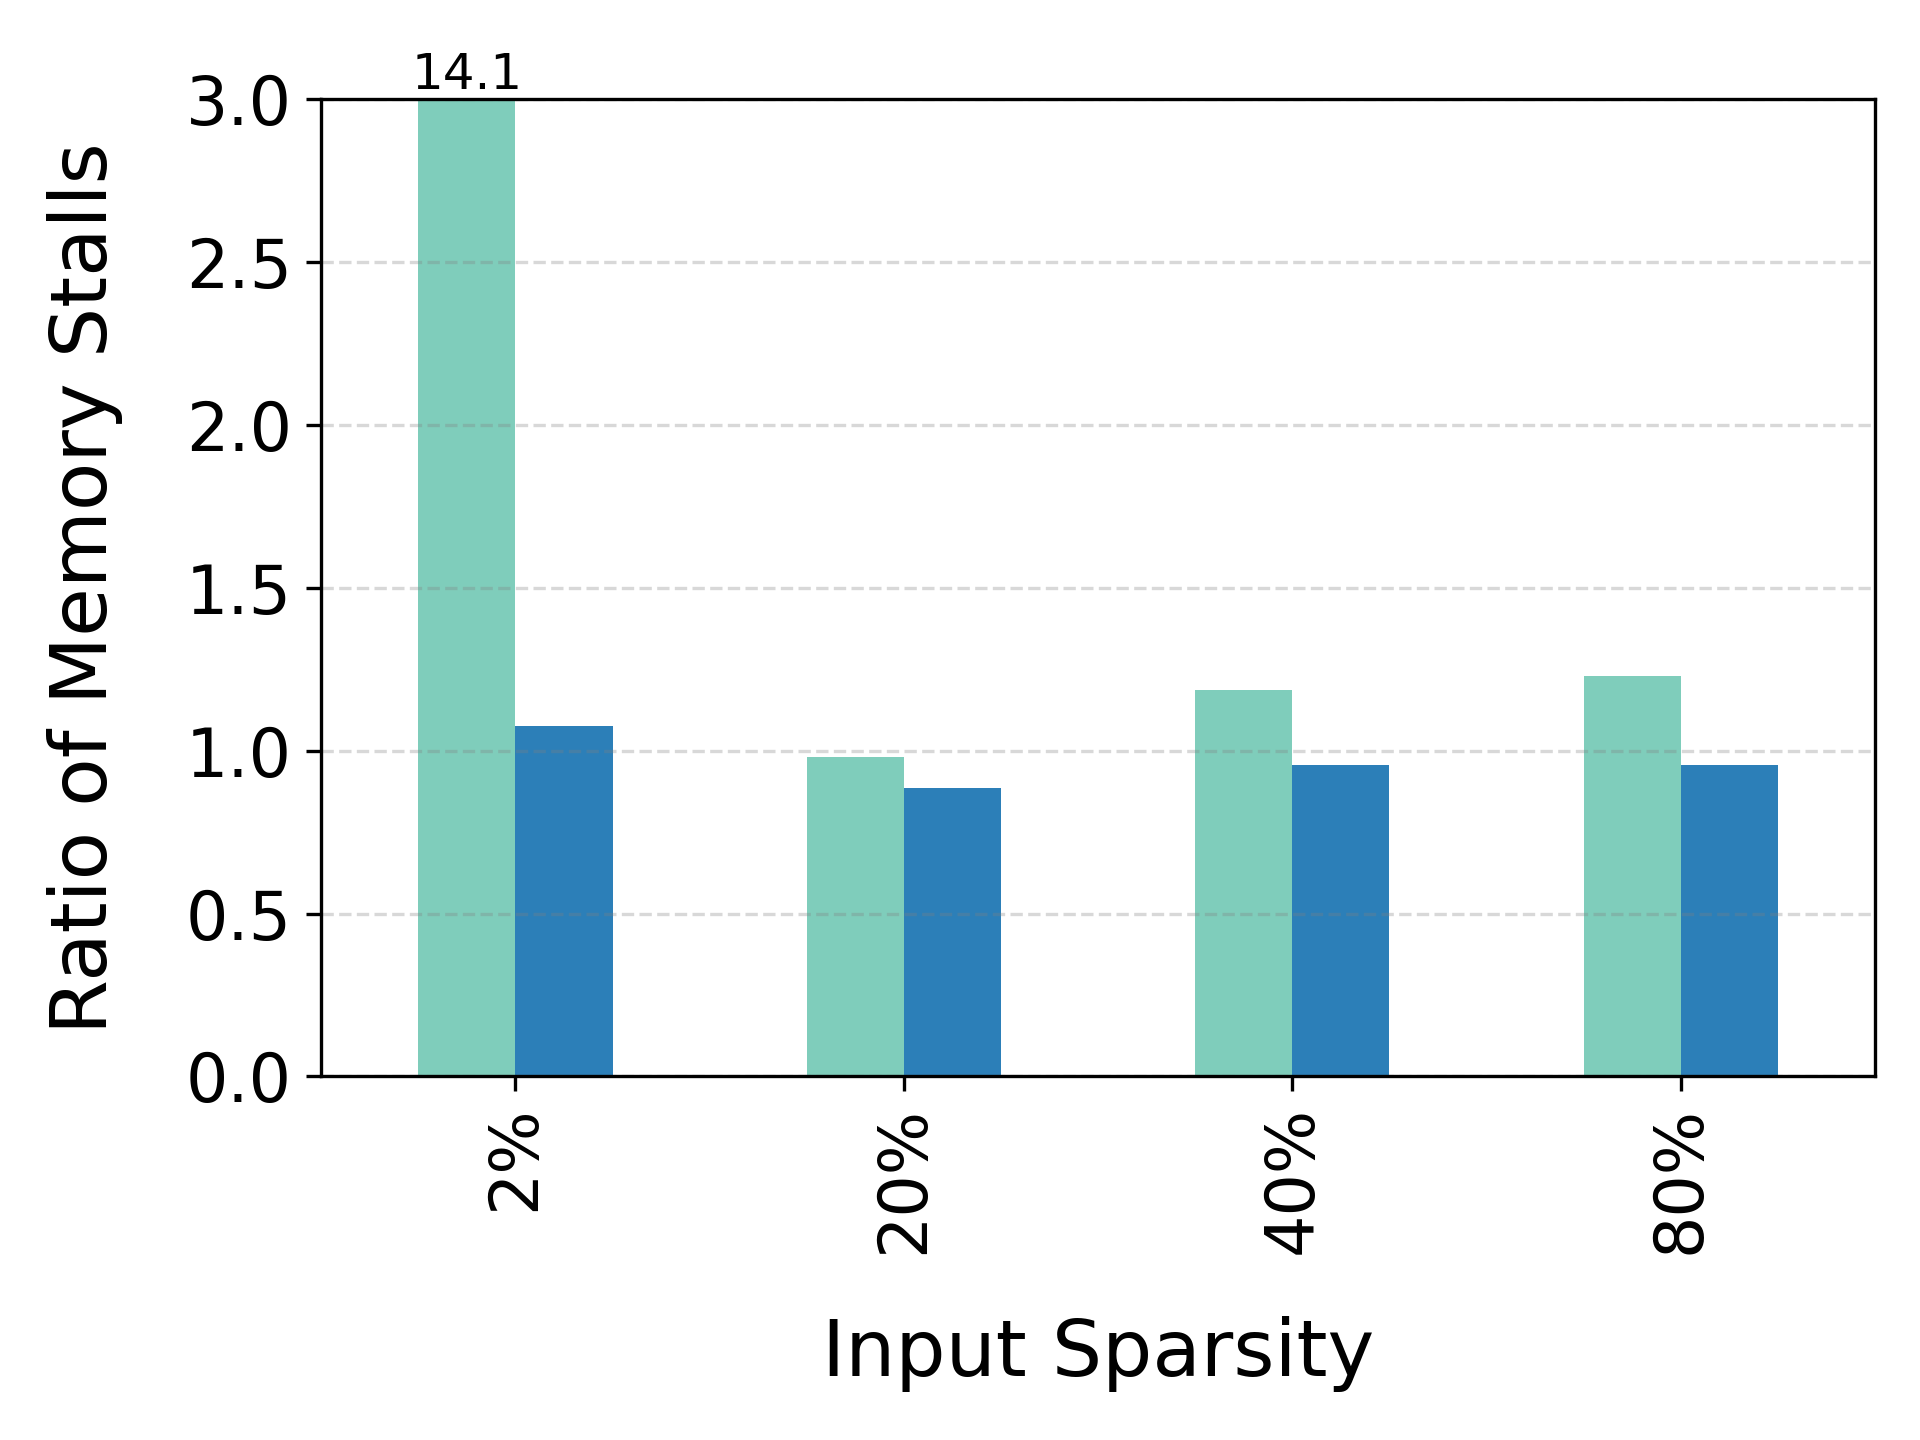
\includegraphics[width=\textwidth, height=.28\textheight]{Figures/Evaluations/single_if_few_scatter_mem_stalls.png}
    \caption{Ratio of memory-induced stalls.}
    \label{fig:single-if-few-scatter-mem-stalls}
  \end{subfigure}%
  \caption{Evaluation of the \ifElseBench micro-benchmark modified to have fewer store instructions. All metrics are normalized with respect to \ifconverted code (\ifconv).}
\end{figure*}


As seen in \rfig{single-if-few-scatter-speedup}, even in a modified version of \ifThenBench with fewer store instructions, neither version of ALC can outperform \ifconv.
The exception is the very sparse case ($2\%$), where \ALCdp provides a speedup of $7\%$ over \ifconv.
Thus, the results indicate that \ALCdp can benefit loops with single \cpath and very few true predicates.
\rfig{single-if-few-scatter-inst} shows that ratio of dynamically executed instructions is very similar to the previous case. 
\ifThenBench, which has fewer stores, has similar behavior in terms of resource and memory stalls, as \rfig{single-if-few-scatter-mem-stalls} and \rfig{single-if-few-scatter-resource-stalls} indicate, as the same benchmark with more store instructions.


\section{Potential of ALC}

To demonstrate the broad applicability of \ALC and how different workloads can benefit from it, we apply the transformation to \emph{Test Suite for Vectorizing Compilers} (TSVC) benchmark \cite{levine1991comparative}. For any loop that we can apply \ALC, we can also apply \datapermutation as a result, in this section whenever we refer to the possibility of applying \ALC, it covers \datapermutation as well.


TSVC is composed of more than a hundred small independent functions, each containing one or more loops with different kinds of control flow. The original benchmark is written in FORTRAN language, but we use a version of it that is rewritten in C language \cite{tsvc2}. The benchmark is developed to assess the compiler's capability to apply vectorization to individual loops. Loops in this benchmark are constructed to address several challenges that a compiler might face while trying to vectorize a code, which include: different types of loop-carried dependency, complicated control flow structures, and different memory access patterns. 

While TSVC carefully examines compiler ability for vectorization, it is not a suitable benchmark for measuring performance improvements. Functions in this benchmark do not represent real-world scenarios and are only constructed to introduce challenges for the compiler during vectorization. Loops are small and most of them include a few instructions. Thus, in this experiment, we only report the success and failure of different transformations.

\begin{table}[htbp]
  \centering
  \begin{tabular}{|c|c|c|c|}
    \hline
    \textbf{Function} & \textbf{GCC} & \textbf{Arm's Clang} & \textbf{ALC+DP} \\
    \hline
        s123  & \texttimes& \texttimes& \texttimes \\
        s124  & \checkmark& \checkmark& \texttimes \\
        s161  & \checkmark& \texttimes& \texttimes \\
        s1161 & \texttimes& \texttimes& \texttimes \\
        s253  & \checkmark& \checkmark& \checkmark \\
        s258  & \texttimes& \texttimes& \texttimes \\
        s271  & \checkmark& \checkmark& \checkmark \\
        s272  & \checkmark& \checkmark& \checkmark \\
        s273  & \checkmark& \checkmark& \checkmark \\
        s274  & \checkmark& \checkmark& \checkmark \\
        s278  & \checkmark& \checkmark& \texttimes \\
        s2710 & \texttimes& \checkmark& \checkmark \\
        s2711 & \checkmark& \checkmark& \checkmark \\
        s2712 & \checkmark& \checkmark& \checkmark \\
        s314 & \texttimes& \texttimes& \texttimes \\
        s315 & \texttimes& \texttimes& \texttimes \\
        s316 & \texttimes& \texttimes& \texttimes \\
        s318 & \texttimes& \texttimes& \texttimes \\
        s3110 & \texttimes& \texttimes& \texttimes \\
        s13110 & \texttimes& \texttimes& \texttimes \\
        s3111 & \checkmark& \texttimes& \texttimes \\
        s3113 & \texttimes& \texttimes& \texttimes \\
        s331 & \checkmark& \texttimes& \texttimes \\
        s341 & \texttimes& \texttimes& \texttimes \\
        s342 & \texttimes& \texttimes& \texttimes \\
        s343 & \texttimes& \texttimes& \texttimes \\
        s443 & \checkmark& \checkmark& \texttimes \\
        vif & \checkmark& \checkmark& \checkmark \\
    \hline
        Total Vectorized & 14 & 12 & 9\\
    \hline
  \end{tabular}
  \caption{Comparison between ALC and state-of-the-art compilers on their ability to vectorize functions of TSVC benchmark}
  \label{tab:tsvc}

\end{table}

Among all functions in the benchmark, there are 29 functions that contain loops with 2 control-flow paths. aWe evaluate the applicability of our approach to them. For each function, we try to apply ALC and compare it with 2 state-of-the-art compilers. We compare against GCC version 13.1.0 and Arm's Clang version 22.1. For each compiler, we pass all flags that enable vectorization and those that enable the compiler to utilize SVE instructions. 

Results are summarized in \rtab{tsvc}. ALC can be applied to most cases that commercial compilers can vectorize. For most cases in which all compilers fail to vectorize --- and where it is not possible to apply ALC as well, the loops contain loop-carried dependencies. While \gcc showed the highest level of efficiency by vectorizing 14 functions out of 29, it failed to vectorize micro-benchmarks that we used for analyzing the performance of generated codes in \rsec{setup}. It was also not able to vectorize some of the masked memory operations and thus, the whole loop was not vectorized.

There are three functions that both \gcc and \armclang are able to vectorize but \ALC fails. The reason why \ALC is not applied in \code{s124} is because of the loop induction variable. Although there is a single loop, it contains two different induction variables, which are both incremented in each iteration of the loop. Although it is not a problematic case for \ALC algorithm to handle, the current implementation considers that all memory accesses are only dependent on the canonical induction variable of the loop.




\begin{center}
\begin{minipage}[t]{0.99\columnwidth}
\begin{lstlisting}[
escapechar=|,
style=code_snippet_style,
language=C,
caption={Simpilifed version of the loop in s278 function},
label=lst:s278]
for (int i = 0, j = 0; i < n; i++) {
    if (...) { 
        b[i] = ....
    }else{
        c[i] = ....
    }
    ... = b[i] + c[i] * ....
}
\end{lstlisting} 
\end{minipage}
\end{center}

The loop in \code{s278} is a more challenging case for \ALC. \rlst{s278} shows the dependency that exists in the loop on arrays \code{b} and \code{c}: in each iteration, there is a write to either \code{b} or \code{c} array (lines 3 and 5), but then there is always a read from each one (line 7). Thus, whenever execution reaches line 7, it must have updated the value that is stored in the corresponding index for array \code{a} or \code{b}. After vectorization by If-Conversion, this pattern is kept and the order of the instructions does not change, however, \ALC does not guarantee that all stores to \code{b} or \code{c} are completed before reaching line 7 because \ALC only executes the \code{then} or \code{else} blocks after it forms a fully uniform vector. Based on the algorithm, in each iteration only one of these two blocks will be executed and one of those two arrays will not be updated by the time that the load instructions of line 7 get executed. 

\begin{center}
\begin{minipage}[t]{0.99\columnwidth}
\begin{lstlisting}[
escapechar=|,
style=code_snippet_style,
language=C,
caption={Simpilifed version of the loop in 443 function},
label=lst:s443]
for (int i = 0, j = 0; i < n; i++) {
    if (...) { 
        a[i] += b[i] * c[i];
    }else{
        a[i] += b[i] * b[i];
    }
}
\end{lstlisting} 
\end{minipage}
\end{center}

Clang uses \textbf{sink} optimization to avoid copies of similar instructions on paths with a common post-dominator. In the loop with an if-then-else statement in \rlst{s443} each of those two blocks contains a write instruction to array \code{a}. The loop is optimized by calculating values (\code{a[i]+ b[i] * c[i]}) and (\code{a[i] + b[i] * b[i]}) in their corresponding blocks, but the actual store to \code{a} happens after the \code{else} block, using a PHI node to determine the right value. \ALC cannot be applied in this case because the current implementation relies on PHI nodes to identify divergent values to generate the permutation logic. A future implementation could address the problem by undoing the sink of stores or by having a more robust mechanism to distinguish data from control divergence.



\begin{center}
\begin{minipage}[t]{0.99\columnwidth}
\begin{lstlisting}[
escapechar=|,
language=C,
style=code_snippet_style,
caption={Loop-carried dependency in s161 function},
label=lst:s161]
for (int i = 0, j = 0; i < n; i++) {
    if (...) { 
        c[i+1] = ....
    }else{
        .... = c[i] + ...
    }
}
\end{lstlisting} 
\end{minipage}
\end{center}

\code{s161} is a very interesting case. Only \gcc is able to vectorize the code and both \armclang and \ALC fail. The reason is loop-carried dependency.
\rlst{s161} shows a simplified version of the code. As demonstrated, there is a write-after-read dependency on array \code{c}. In the \code{then} block, \code{c[i+1]} is being written to, and in the \code{else} block \code{c[i]} it is being read. When vectorizing this kind of dependency, if we can make sure that write operations are done before read operations, vectorization will be legal. 
\nelson{The next sentence is not grammatically correct.}
In this case,  the write and read operations are placed in two different blocks, and they can be safely reordered during vectorization as conditions are mutually exclusive as a result, vectorization is allowed.

\nelson{The next sentence is not grammatically correct.}

\gcc detected the legality of vectorizing \code{s161} under this condition however, \armclang failed to find the opportunity. \ALC cannot be applied in this case because, as discussed before, it cannot guarantee the order in which the \code{then} and the \code{else} blocks are executed.

\code{s2710} is the case where \armclang and \ALC outperform \gcc. While the function is vectorized by \armclang and \ALC is also applied, \gcc fails to vectorize the code due to the presence of complex control flow inside the loop. The control flow consists of two-level nested if-then-else statements: there is another if-then-else inside both then and else blocks. \code{Armclang} finds that the loop can be broken into two simpler loops each having only one if-then-else (a common compiler optimization called loop fission) and by doing so, it can vectorize both loops. Having these two simpler loops, \ALC is also able to transform both of them but \gcc fails to find the opportunity to simplify and vectorize the code.

The loops in \code{s314, s315, s316, s318, s3110, s13110, s311, s3113} functions contain code structures that require employing a \textbf{Reduction} technique for vectorization. 
Examples of reduction operations include: computing the sum, the product, the maximum value, or the minimum value of all the elements of a loop. In all these cases there is a scalar value that creates a loop-carried dependence in the scalar code. This dependence prevents vectorization. However, using the reduction technique, the compiler is able to vectorize such loops. As shown in \rtab{tsvc} \gcc, \armclang and \ALC fail on most reduction cases. In fact, only \gcc is able to vectorize \code{s311} which is a simple summation of elements of an array.

\code{331} contains a search loop where the goal is to find the index of the last element which is smaller than zero. \gcc vectorizes the code using techniques similar to reduction but \armclang and \ALC are not able to transform the code.

In summary, although \gcc vectorizes a few more functions, both compilers perform close to each other. \ALC can be applied in the majority of cases where vectorization is allowed and possible, which indicates that there are many use cases where different programs can benefit from it. 

\section{Conditionally Incremented Array Indexes}
\label{sec:eval-limitations}

The ALC analysis pass found many loops in existing benchmarks (e.g. SPEC CPU 2017~\cite{spec} and MiBench~\cite{MiBench}) that could be legally transformed by ALC transformation.
However, the cost/benefit analysis indicated that those loops would not benefit from ALC because they contained not enough instructions to amortize the cost of index and data permutation (see \rsec{alc-analysis}).



Another challenge discovered when trying to apply ALC to existing benchmarks that contain loops with conditional statements, such as the ones in MiBench~\cite{MiBench}, is related to efficient mappings of conditional computations to vector code. 


\begin{center}
\begin{minipage}[t]{0.99\columnwidth}
\begin{lstlisting}[
escapechar=|,
style=code_snippet_style,
language=C,
caption={Conditional increment of array indexing variable.},
label=lst:cond-indvar]
for (int i = 0, j = 0; i < n; i++) {
    if (cond[i]) { |\label{lst:cond-indvar:cond}|
        b[i] = a[j];
        j++; |\label{lst:cond-indvar:j-inc}|
    }
}
\end{lstlisting} 
\end{minipage}
\end{center}

For example, \rlst{cond-indvar} shows a simplified example of a loop pattern that is widely found in the \code{jpeg} benchmark in MiBench.
The loop index into array \code{a} with variable \code{j}, which is conditionally incremented when (\rline{cond-indvar:j-inc}) \code{cond[i]} is true (\rline{cond-indvar:cond}).
To the best of our knowledge, there is no single instruction in modern vector ISAs that can \textit{efficiently} compute an index vector with the values of \code{j} in this case.
Therefore, multiple instructions are required, which might make it unprofitable to vectorize such loops.
Neither Clang, GCC, nor Arm's Clang vectorized the loops in SPEC CPU 2017 with the pattern shown in \rlst{cond-indvar}.
These non-trivially vectorizable patterns led this work to not find opportunities to apply ALC as a compiler-enabled transformation to these benchmark suites.
If future versions of vector ISAs include instructions to create conditionally-strided index vectors then more loops could become candidates for \ifconversion and ALC.
A potential workaround would be to compute the values of \code{j} on a separate loop, storing such values in a temporary array, and then using the computed array to index \code{a}.
However, hoisting the computation might not always be possible because of intra-iteration dependencies.
